% =============================================================================
% BioSeqInsight 2.0 manuscript
% Target: Bioinformatics Advances (Original Article) / backup: PLOS ONE
% -----------------------------------------------------------------------------
% This is intentionally written against a generic article class rather than
% the OUP bioinfo.cls or the PLOS LaTeX template, on the explicit instruction
% that formatting/length will be adapted per-journal afterwards. All content,
% section structure and citations are written to be portable to either
% target with mechanical reformatting (class swap + \bibliographystyle
% change) rather than a rewrite.
%
% To compile:
%   pdflatex main && bibtex main && pdflatex main && pdflatex main
% =============================================================================

\documentclass[11pt]{article}

% ---- packages ---------------------------------------------------------------
\usepackage[margin=1in]{geometry}
\usepackage[utf8]{inputenc}
\usepackage[T1]{fontenc}
\usepackage{amsmath,amssymb}
\usepackage[expansion=false]{microtype}
\usepackage{graphicx}
\usepackage{booktabs}
\usepackage{array}
\usepackage{longtable}
\usepackage{xcolor}
\usepackage{tikz}
\usetikzlibrary{arrows.meta, positioning, fit, backgrounds, shapes.geometric}
\usepackage{authblk}
\usepackage[colorlinks=true, linkcolor=blue!50!black, citecolor=blue!50!black,
            urlcolor=blue!50!black]{hyperref}
\usepackage{natbib}
\bibliographystyle{unsrtnat}
\usepackage{caption}
\captionsetup{font=small, labelfont=bf}
\usepackage{enumitem}
\usepackage{listings}
\usepackage{fancyvrb}
\usepackage{lineno}
\usepackage{setspace}
\usepackage{todonotes}

% Monospace listing style for CLI examples / code
\lstdefinestyle{cli}{
  basicstyle=\ttfamily\small,
  breaklines=true,
  columns=fullflexible,
  frame=single,
  backgroundcolor=\color{gray!8},
  rulecolor=\color{gray!40}
}
\lstset{style=cli}

% Mapping-level colour macros, used consistently in text, tables and figures
\definecolor{mapM4}{HTML}{1a7f37}
\definecolor{mapM3}{HTML}{0969da}
\definecolor{mapM2}{HTML}{9a6700}
\definecolor{mapM1}{HTML}{cf222e}
\definecolor{mapM0}{HTML}{6e7781}
\newcommand{\mlevel}[1]{\textbf{#1}}

\newcommand{\bsi}{\textsc{BioSeqInsight}}
\providecommand{\provisionalbanner}{}
\InputIfFileExists{results/numbers}{}{\providecommand{\N}[1]{\textbf{??}}}
\newcommand{\todoinline}[1]{\todo[inline, backgroundcolor=yellow!30]{#1}}

\linenumbers % remove for camera-ready; helpful for reviewers

\title{\bsi\ 2.0: An Integrated Desktop Platform for DNA Sequence Analysis
with Validated Protein Structure-Resource Retrieval}

% -----------------------------------------------------------------------------
% AUTHOR BLOCK -- placeholder. Needs real names, affiliations, ORCID iDs and
% the corresponding-author email before submission. See the accompanying
% message for exactly what is needed here.
% -----------------------------------------------------------------------------
\author[1]{Author Name\thanks{Corresponding author: \texttt{email@institution.edu}}}
\affil[1]{Department/Institution, City, Country}

\date{}

\begin{document}
\maketitle
\provisionalbanner

\begin{abstract}
\textbf{Motivation:} Moving from a nucleotide sequence to a protein structure
usually means chaining independent web tools, and the step that would confirm
that a retrieved structure is the queried molecule is easily skipped, because a
sequence search returns similar sequences, not necessarily the one asked about.
How often a naive workflow returns the wrong structure has rarely been measured.

\textbf{Results:} We present \bsi\ 2.0, a desktop and command-line platform that
integrates sequence analysis (ORF finding, translation, protein properties,
primer thermodynamics) with structure retrieval from RCSB PDB, AlphaFold DB and
ESM Atlas. Every retrieved structure is aligned to the query and its database
cross-references are checked, and the result is reported on a five-level scale
(M0--M4) in which only a full-length, accession-confirmed match is M4; a
confirmed but incomplete structure is flagged as partial. We measured the effect
on \N{ds-n} randomly sampled reviewed UniProt proteins from \N{ds-orgs}
organisms, judged against curated PDBe SIFTS and RCSB cross-references rather
than against our own alignment. Accepting the top RCSB sequence-search hit
returned a structure not catalogued under the queried accession for
\N{n1-all-false} of \N{n1-all-q} queries, including \N{n1-has-false} of
\N{n1-has-acc} hits (\N{n1-has-far}\%) for the \N{ds-has} proteins that have a
deposited structure; \N{n1-all-tier-diff} of the \N{n1-all-false} were
$<$90\% identical to the query. Accepting only M4 gave \N{s1-all-false} false
associations among \N{s1-all-acc} accepted structures (95\% CI
\N{s1-all-far-lo}--\N{s1-all-far-hi}\%) but returned a correct structure for
\N{s1-has-sens}\% of proteins that have one, against \N{n1-has-sens}\% for the
naive policy; of the \N{gate-rejected} correct hits it rejected, \N{gate-partial}
were partial structures and \N{gate-unmeasured} could not be validated because no
PDB-format file exists. Constructed negatives (unrelated proteins, fragments,
paralogues) reached M4 in \N{adv-nonB3-M4} of \N{adv-nonB3-n} cases. The M2
threshold is not evidence of homology: \N{nf-m2-pct}\% of unrelated pairs satisfy
it. Engineering evidence includes 502 automated tests, deterministic fault
injection (80.0\% recovery of injected faults), and a reduction from 849 to 14
user interaction steps against a documented manual workflow.

\textbf{Availability:} \bsi\ is implemented in Python (standard library only for
its core computations), released under the MIT licence, and available at
\url{https://github.com/niloy-999/BioSeqInsight}
(\todoinline{Zenodo DOI: XXXX}).

\end{abstract}

\noindent\textbf{Keywords:} bioinformatics software; sequence analysis;
protein structure retrieval; structure validation; reproducibility;
AlphaFold; RCSB PDB; UniProt

\vspace{1em}
\hrule
\vspace{1em}

\section{Introduction}
\label{sec:introduction}

A routine task in molecular biology is to characterise a nucleotide or protein
sequence and then look at the three-dimensional structure of the protein it
encodes. In practice this is a chain of separate tools: a sequence-analysis
package for open reading frames and composition, a primer-design page, a protein
property calculator, and then one or more structure resources, namely the
experimental archive RCSB PDB \citep{berman2000pdb}, the predicted-model
database AlphaFold DB \citep{varadi2022alphafolddb,jumper2021alphafold}, and the
language-model predictor ESM Atlas \citep{lin2023esmfold}. Each hand-off is a
manual copy-and-paste, and each is a place where an identifier can be
mistyped or a result misread.

The step that is most easily skipped is the one that matters most for the
conclusion drawn from a structure: confirming that the structure that came back
is the protein that was asked about. A sequence search is designed to return
\emph{similar} sequences, and the structure archives are keyed in different
ways: AlphaFold DB by UniProt accession, RCSB PDB by entry and by sequence
similarity, ESM Atlas by predicting from the sequence alone. A hit therefore
tells the user that something was found, not that it is the queried molecule: it
may be a paralogue, a fragment, a different isoform, or the same protein
catalogued under a different accession. Scripts that fetch ``the first
structure'' and report success make this distinction invisible, and the question
of how often it matters has, to our knowledge, rarely been measured.

This paper has two parts. The first is a software contribution. \bsi\ 2.0
integrates sequence analysis with structure retrieval and, for every retrieved
structure, performs the check that is usually skipped: the structure's chain is
aligned to the query, the structure's own database cross-references are compared
with the queried accession, and the outcome is reported on an explicit five-level
scale (M0--M4) in which only a full-length structure whose accession is confirmed
is called an exact match (Section~\ref{sec:m0m4}). The second is a measurement.
Using \N{ds-n} randomly sampled reviewed UniProt proteins from \N{ds-orgs}
organisms, we ask how often accepting the top sequence-search hit returns a
structure that is not catalogued under the queried accession, how often the
validation layer prevents that, what it costs in correct structures rejected,
and where its thresholds are and are not meaningful
(Section~\ref{sec:validation-study}). Correctness is judged against curated
cross-references from PDBe SIFTS and RCSB rather than against the software's own
alignment, so the evaluation does not simply restate the classifier's output.

A note on how this study came to be framed, because it changed the paper. An
earlier prototype of this software (v1.0) reported a structural hit for every
query in its small benchmark, and its own report flagged that for 7 of 25
queries the UniProt accession attached to the hit differed from the query.
v1.0 had no step that compared the retrieved structure with the query sequence,
so it could not say whether those hits were wrong. We initially read the flags
as failures. Re-adjudicating all 25 queries against current data
(Section~\ref{sec:case-study}) shows that for \N{cs-disc-contains} of the
\N{cs-disc-n} flagged queries the top RCSB sequence-search hit is an entry that
does contain the queried accession (\N{cs-disc-M4} validate as M4), so the
discordance reflected how accessions were attributed to hits, not wrong structures. The lesson we take is methodological:
an accession mismatch in a reporting layer is not the same thing as a wrong
structure, and the two should be separated by an explicit sequence and
cross-reference check on a large sample, which is what the present study does.

\paragraph{Contributions.}
(i) An integrated, dependency-light platform with a command-line and a graphical
interface (Sections~\ref{sec:architecture}--\ref{sec:export}).
(ii) A five-level sequence-to-structure classification with a partial-structure
qualifier, applied uniformly to three heterogeneous resources
(Section~\ref{sec:m0m4}).
(iii) A measurement on \N{ds-n} random proteins of how often naive retrieval
returns a structure not catalogued under the queried accession, how often
validation prevents it, and what that costs
(Section~\ref{sec:validation-study}), with an adversarial benchmark of
constructed negatives (Section~\ref{sec:adversarial}).
(iv) Engineering evidence: an offline test suite, deterministic fault
injection, cross-validation against an established implementation, performance
measurements and an interaction-cost comparison
(Sections~\ref{sec:testing}--\ref{sec:workflow-comparison}).

\section{Related work}
\label{sec:related-work}

\subsection{Sequence-analysis toolkits}

Biopython \citep{cock2009biopython} is the de facto standard Python library
for sequence parsing, translation, and protein-parameter calculation, and is
used directly by a large fraction of bioinformatics scripting in Python.
EMBOSS \citep{rice2000emboss} provides an equivalent, broader suite as
command-line Unix tools rather than a library, including its own
isoelectric-point calculator (\texttt{iep}) and pairwise alignment tools. Both
are mature, well-validated, and neither is superseded by the present work:
\bsi\ reimplements a comparable set of sequence and protein calculations
independently, in pure Python with no required dependencies
(Section~\ref{sec:core-calculations}), and cross-validates that
reimplementation against Biopython directly rather than depending on it, for
reasons discussed in Section~\ref{sec:architecture}. Where the two
deliberately disagree -- most notably on isoelectric point, where no single
pKa scale is universally agreed and independent calculators are documented
to differ by several tenths of a pH unit \citep{kozlowski2016ipc} -- \bsi\
reports the method and conditions used rather than asserting an
unqualified value, and its test suite documents the disagreement rather than
concealing it.

Neither Biopython nor EMBOSS provides an interactive desktop interface, and
neither couples sequence analysis to structure retrieval: a user who wants
both must write connecting code themselves. Several general-purpose
scientific notebook environments (Jupyter-based pipelines built on Biopython)
fill this gap on a per-project basis, but do not constitute a reusable,
tested, packaged tool.

\subsection{Structure databases and prediction resources}

The RCSB Protein Data Bank \citep{berman2000pdb} is the primary repository of
experimentally determined structures and exposes a sequence-search API that
\bsi\ uses directly. The AlphaFold Protein Structure Database
\citep{varadi2022alphafolddb}, built on the AlphaFold prediction method
\citep{jumper2021alphafold}, and the ESM Atlas fold service, built on the
ESMFold language model \citep{lin2023esmfold}, both provide predicted
structures for sequences with no experimental structure, at the cost of a
confidence estimate (predicted local distance difference test, pLDDT) in
place of the crystallographic or cryo-EM validation an experimental
structure carries. \bsi\ does not implement, retrain, or redistribute any of
these prediction methods; it is a client that queries their public APIs,
distinguishes their confidence metric from the superficially similar
crystallographic B-factor reported by experimental structures
(Section~\ref{sec:validation}), and attributes results to the resource that
produced them. None of the three resources' own interfaces performs the
identity check described in Section~\ref{sec:m0m4} against an
externally supplied query sequence; that check is outside their scope as
databases, and is precisely the gap this software is built to close for a
client performing automated or semi-automated retrieval.

\subsection{Structure visualisation and analysis tools}

PyMOL \citep{pymol}, UCSF ChimeraX \citep{pettersen2021chimerax}, and web-based
viewers such as 3Dmol.js \citep{rego20153dmol} provide structure
visualisation and, in the case of PyMOL and ChimeraX, extensive structural
analysis capability once a coordinate file has been obtained. \bsi\ embeds
3Dmol.js for in-application viewing and can hand a retrieved structure to an
external viewer such as PyMOL or ChimeraX when one is installed
(Section~\ref{sec:gui}), rather than duplicating their visualisation or
analysis functionality. Its contribution is upstream of visualisation:
deciding, before a structure is opened in any viewer, whether it is the
structure the user actually asked for.

\subsection{Positioning}

\bsi\ does not claim algorithmic novelty in its sequence alignment, which
uses standard Needleman--Wunsch and semi-global dynamic programming
\citep{needleman1970}, nor in its thermodynamic and physicochemical
calculations, which follow established published methods
(Sections~\ref{sec:core-calculations}--\ref{sec:validation}). Its
contribution is threefold and specifically evidentiary rather than
algorithmic: (i) an explicit, thresholded classification of
sequence-to-structure correspondence (M0--M4) applied uniformly across
three heterogeneous structural resources, in place of the implicit
binary success/failure result common to ad hoc retrieval scripts and to the
initial prototype of this software, whose benchmark reported a hit for every query; (ii) an integrated workflow in which
sequence analysis, structure retrieval, and validation share one
configuration, one cache, and one reproducible project record, rather than
requiring a user to coordinate several independent tools by hand; and (iii)
a body of evidence -- an offline test suite, deterministic fault injection,
cross-validation against Biopython, and a measurement of how often naive
retrieval returns the wrong structure for \N{ds-n} randomly sampled proteins,
judged against independently curated cross-references, together with an
adversarial benchmark -- supporting the reliability of that classification and
reporting its cost and its limits.

\section{Methods}
\label{sec:methods}

\subsection{System architecture}
\label{sec:architecture}

\bsi\ is organised as a layered Python package with dependencies enforced
to point in a single direction, shown in Figure~\ref{fig:architecture}. A
\texttt{core} layer implements every nucleotide and protein calculation
against the Python standard library only, with no file, network, or
graphical-interface access. A \texttt{models} layer defines typed,
JSON-serialisable result dataclasses shared by every layer above it,
replacing the pattern -- present in the initial prototype -- of returning
pre-formatted display strings directly from analysis functions, which
precludes batch processing, machine-readable export, and independent testing
of computed values versus displayed wording. A \texttt{services} layer
provides HTTP transport (with pluggable backends, Section~\ref{sec:testing}),
a retry policy, an on-disk response cache, and structured logging. A
\texttt{structures} layer implements one client class per external resource
(RCSB, AlphaFold DB, ESM Atlas, UniProt) plus the validation logic of
Section~\ref{sec:validation} and a manager that sequences providers
according to configurable fallback order. A \texttt{workflows} layer
implements batch analysis and reproducible project management
(Section~\ref{sec:reproducibility}). An \texttt{io} layer implements CSV,
TSV, JSON, and self-contained HTML export. Finally, a command-line interface
and a Tkinter graphical interface both consume the same underlying API,
described in Section~\ref{sec:implementation}.

\begin{figure}[htbp]
\centering
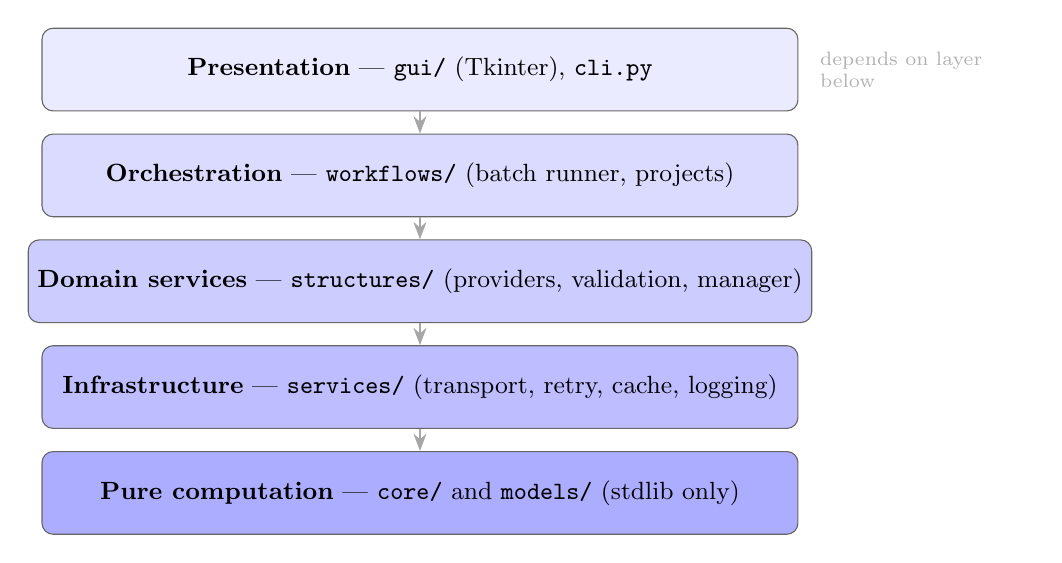
\begin{tikzpicture}[
    layer/.style={rectangle, rounded corners, draw=black!60, minimum width=9.6cm,
                  minimum height=1.05cm, align=center, font=\small},
    arrow/.style={-{Stealth[length=2.2mm]}, thick, gray!70}
  ]
  \node[layer, fill=blue!8]  (gui)  {\textbf{Presentation} --- \texttt{gui/} (Tkinter), \texttt{cli.py}};
  \node[layer, fill=blue!14, below=0.28cm of gui]  (wf)   {\textbf{Orchestration} --- \texttt{workflows/} (batch runner, projects)};
  \node[layer, fill=blue!20, below=0.28cm of wf]   (str)  {\textbf{Domain services} --- \texttt{structures/} (providers, validation, manager)};
  \node[layer, fill=blue!26, below=0.28cm of str]  (svc)  {\textbf{Infrastructure} --- \texttt{services/} (transport, retry, cache, logging)};
  \node[layer, fill=blue!32, below=0.28cm of svc]  (core) {\textbf{Pure computation} --- \texttt{core/} and \texttt{models/} (stdlib only)};

  \draw[arrow] (gui.south) -- (wf.north);
  \draw[arrow] (wf.south) -- (str.north);
  \draw[arrow] (str.south) -- (svc.north);
  \draw[arrow] (svc.south) -- (core.north);

  \node[right=0.15cm of gui, font=\scriptsize, text width=2.6cm, align=left, text=gray!60]
       {depends on layer below};
\end{tikzpicture}
\caption{\bsi\ layer architecture. Dependencies point downward only;
\texttt{core} imports nothing outside the Python standard library, which is
verified by a dedicated continuous-integration job that installs the package
with no optional extras and fails if a third-party import is reachable from
\texttt{core}.}
\label{fig:architecture}
\end{figure}

Three design decisions follow directly from the motivating problem in
Section~\ref{sec:introduction}. First, results are dataclasses rather than
formatted strings, so that the value a validation check acts upon and the
text a user reads are produced from the same computation and can be tested
independently; the wording shown in the interfaces, including every warning
that accompanies a non-exact structure match, is itself covered by tests
(Section~\ref{sec:testing}). Second, sequence-to-structure validation
(Section~\ref{sec:validation}) is implemented as a single function called
uniformly by the manager after every provider returns a result, rather than
being available as an opt-in utility a caller might omit -- the failure mode
in Section~\ref{sec:introduction} arose precisely because validation was
optional in the initial prototype. Third, the HTTP transport is an
interface with three implementations (a \texttt{requests}-based transport,
a standard-library \texttt{urllib} transport used when \texttt{requests} is
not installed, and a scripted fake transport used only in tests), which is
what makes deterministic fault-injection testing possible
(Section~\ref{sec:fault-injection}): a test can assert that two HTTP 504
responses followed by a 200 response produce exactly one recovered result,
on every machine, without depending on a real service failing at a
convenient moment.

\subsection{DNA and protein sequence analysis}
\label{sec:core-calculations}

\paragraph{Nucleotide analysis.}
Input sequences are accepted in FASTA or raw form; header lines, whitespace,
and non-nucleotide punctuation copied incidentally from database records
(digits, alignment gaps) are ignored, while genuine unexpected symbols are
reported rather than silently discarded. Reported nucleotide measures
include base composition and GC content (IUPAC ambiguity codes excluded from
both numerator and denominator, so that a sequence with unresolved bases is
not artificially reported as GC-poor), reverse complementation, transcription,
six-frame translation, open-reading-frame detection with a configurable
minimum length and choice of NCBI genetic code table (standard, vertebrate
mitochondrial, mould/protozoan mitochondrial, and bacterial/archaeal tables
are bundled), and IUPAC degenerate-motif search on both strands.
Ambiguity codes are retained in place during translation rather than
stripped before codon splitting: a codon containing an unresolved base
translates to an unspecified residue (\texttt{X}) at its own position,
which preserves the reading frame of every downstream codon. Melting
temperature is estimated by the Wallace rule for short oligonucleotides and
by SantaLucia's nearest-neighbour thermodynamics with salt correction
\citep{santalucia1998} for longer duplexes within the range for which that
two-state model is applicable; the method and the primer/salt conditions
used are always reported alongside the value, and a duplex outside the
model's validated length range carries an explicit caveat rather than a bare
number.

\paragraph{Protein analysis.}
Protein descriptors include average molecular weight (IUPAC average residue
masses, less one water molecule per peptide bond), grand average of
hydropathy (GRAVY) and a Kyte--Doolittle hydropathy profile
\citep{kytedoolittle1982}, aromaticity and aliphatic index
\citep{ikai1980aliphatic}, extinction coefficient at 280\,nm by the
Gill--von Hippel method \citep{gillvonhippel1989} (reported both with
cysteines reduced and as cystines), and isoelectric point by iterative
charge-balance search over a Bjellqvist-style pKa table. Because independent
isoelectric-point calculators are documented to disagree by several tenths
of a pH unit depending on which of several published pKa scales they use
\citep{kozlowski2016ipc}, \bsi\ does not claim numerical identity with any
one external tool; instead its cross-validation suite
(Section~\ref{sec:cross-validation}) checks agreement with Biopython within
a stated, literature-consistent tolerance and, independently of any external
tool, checks that the net charge computed at the reported isoelectric point
is itself zero. A Chou--Fasman-style secondary-structure propensity sketch
\citep{choufasman1978} is provided for illustrative and teaching purposes
and is labelled, in the interface, the exported data, and this manuscript,
as a propensity sketch rather than a structure prediction; a user who needs
an actual secondary-structure assignment is directed to DSSP applied to a
real structure, or to a dedicated modern predictor.

\subsection{External structure-resource retrieval}
\label{sec:retrieval}

Three structural resources are queried, each through a dedicated provider
class implementing a common interface (Figure~\ref{fig:architecture}):

\begin{itemize}[leftmargin=1.4em]
  \item \textbf{RCSB PDB} \citep{berman2000pdb}: direct retrieval by PDB
  identifier, or sequence search followed by download of the top-scoring
  entry, with cross-reference accessions read from the matched polymer
  entity's reference-sequence metadata.
  \item \textbf{AlphaFold Protein Structure Database}
  \citep{varadi2022alphafolddb}: retrieval by UniProt accession. The
  provider queries the public prediction API to discover the model file
  currently served for that accession, rather than constructing the file
  URL from an assumed model-version number; the database periodically
  republishes its models under a new version, and a client that instead
  encodes a fixed version number degrades to reporting a coverage gap for
  every accession once the database moves past it, a failure mode that is
  indistinguishable from genuinely absent coverage without querying the
  authoritative endpoint. An HTTP 404 response from the prediction API is
  treated as a true coverage gap and is not retried; a malformed or empty
  API response is treated as a service failure and is.
  \item \textbf{ESM Atlas} (ESMFold, \citealp{lin2023esmfold}): on-demand
  structure prediction from an arbitrary sequence, subject to a configurable
  maximum sequence length; sequences exceeding the limit are rejected before
  any network request is made, and this rejection is reported as its own
  outcome category distinct from either a retrieved structure or a service
  failure (Section~\ref{sec:evaluation}).
\end{itemize}

UniProt \citep{uniprot2023} is queried first when the input is an
accession, to obtain the canonical sequence against which every retrieved
structure is subsequently validated; without this step, an accession query
would have no query sequence for the validation check of
Section~\ref{sec:validation} to use.

Providers are tried in a configurable order (RCSB, then AlphaFold DB, then
ESM Atlas, by default) and the manager stops at the first exact (M4,
Section~\ref{sec:m0m4}) match, unless configured to query every resource
regardless (used for the benchmark in Section~\ref{sec:live-benchmark}).
Responses are cached on disk, keyed by resource, query, and relevant
parameters, with a stored SHA-256 checksum verified before a cached payload
is served; a tampered or corrupted cache entry is discarded and refetched
rather than served.

\subsection{Sequence-to-structure validation}
\label{sec:validation}

Every structure a provider returns is compared against the query sequence
before being reported. The coordinate file is parsed to recover per-chain
sequence (from \texttt{SEQRES} records where present, falling back to the
$\text{C}\alpha$ trace otherwise), and the chain whose sequence aligns best
to the query is selected.

Alignment uses semi-global (``glocal'') dynamic programming rather than a
strict global alignment: the query is aligned end to end while the subject
chain may be a sub-sequence of it with no length penalty. Scoring is
deliberately simple (match $+1$, mismatch $-1$, linear gap $-2$, no
substitution matrix): the alignment's role here is to measure identity and
coverage of one candidate against the query, not to rank distant homologues
by evolutionary score. Because identity is taken over the aligned region only, it
depends on the scoring scheme: with permissive gap scoring, an alignment of two
unrelated sequences can reach a high identity over a short aligned stretch
(Section~\ref{sec:threshold}), so identity is only interpretable together with
coverage and, for the strongest claim, with the accession check. The algorithm has $O(mn)$ time and memory bound guarded by a maximum
cell-count cap that raises an explicit error rather than exhausting memory
on pathologically long inputs. This choice matters concretely: a deposited
construct that omits a cleaved signal peptide or a disordered terminal
region -- common in crystallography -- is still a correct structure of the
folded domain it does cover, and a strict global alignment
\citep{needleman1970} would understate its identity in proportion to the
omitted length. Two measures are reported: \emph{identity}, the fraction of
aligned positions that match, and \emph{coverage}, the fraction of the query
length included in the alignment; a fragment therefore shows high identity
with reduced coverage, which is the correct characterisation, rather than
being scored as a poor match overall.

Accessions are collected from the coordinate file's own cross-references
(\texttt{DBREF} records and equivalent \texttt{REMARK} fields) and, where
the originating provider's API exposes it, from provider-supplied metadata
independent of the coordinate file itself -- for RCSB, the matched polymer
entity's reference-sequence identifiers. The queried accession is
normalised (handling FASTA header forms such as
\texttt{sp\textbar P24941\textbar CDK2\_HUMAN} and AlphaFold model names such
as \texttt{AF-P69905-F1}) and compared against this set.

\subsection{M0--M4 sequence-to-structure correspondence classification}
\label{sec:m0m4}

The identity, coverage, and accession-match measures of
Section~\ref{sec:validation} are combined into a single ordinal
classification, summarised in Table~\ref{tab:m0m4} and
Figure~\ref{fig:decision}, reported alongside every retrieved structure in
both interfaces and in every exported table.

\begin{table}[htbp]
\centering
\small
\caption{The M0--M4 sequence-to-structure correspondence scale. Default
thresholds are shown; all six numeric thresholds are configurable and the
values in force are recorded with every result.}
\label{tab:m0m4}
\begin{tabular}{@{}llp{7.4cm}@{}}
\toprule
\textbf{Level} & \textbf{Name} & \textbf{Criteria} \\
\midrule
\textcolor{mapM4}{\mlevel{M4}} & Exact &
Accession cross-referenced by the structure \emph{and} identity $\geq 99\%$
\emph{and} coverage $\geq 95\%$. \\[2pt]
\textcolor{mapM3}{\mlevel{M3}} & High confidence &
Identity $\geq 95\%$ and coverage $\geq 80\%$; accession not confirmed
(the same or a near-identical sequence). \\[2pt]
\textcolor{mapM2}{\mlevel{M2}} & Related record &
Identity $\geq 40\%$ and coverage $\geq 40\%$, below the M3 thresholds
(a homologue, an orthologue, or a fragment); \emph{not} evidence of homology
(Section~\ref{sec:threshold}). \\[2pt]
\textcolor{mapM1}{\mlevel{M1}} & Unverified &
Either no comparison was possible (no query sequence, or no readable chain),
\emph{or} a comparison was made and fell below even the M2 thresholds. \\[2pt]
\textcolor{mapM0}{\mlevel{M0}} & No result &
No structural record was returned by any queried resource. \\
\bottomrule
\end{tabular}
\end{table}

\begin{figure}[htbp]
\centering
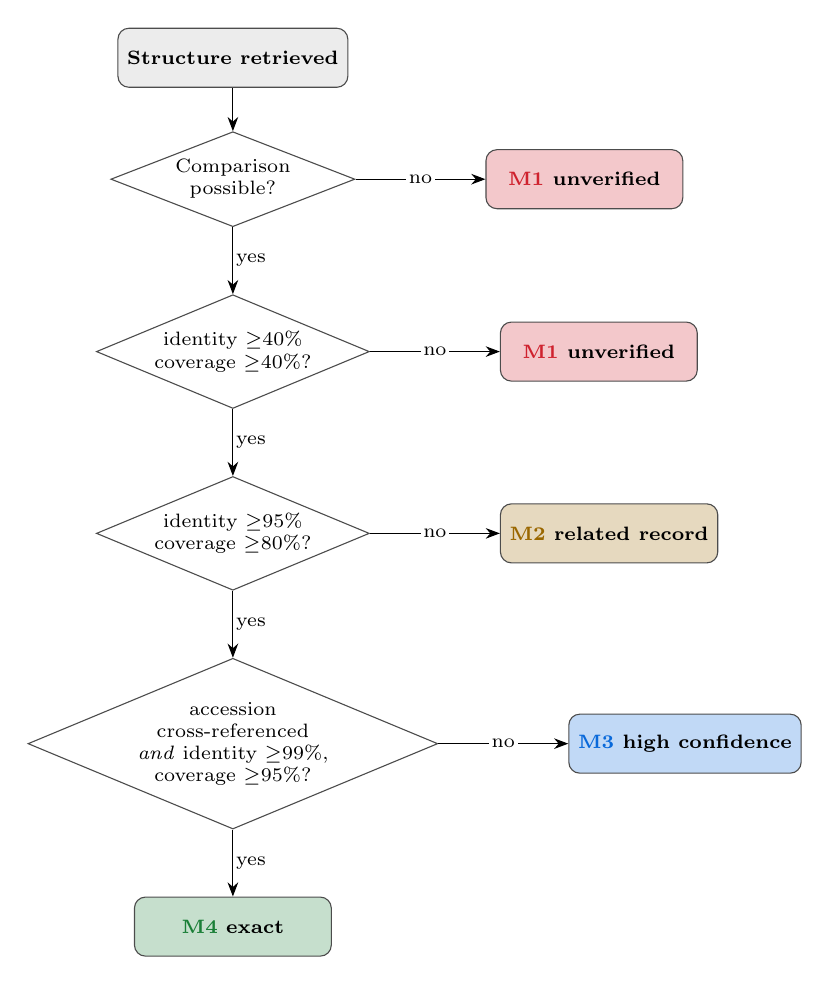
\begin{tikzpicture}[
    dec/.style={diamond, draw=black!70, aspect=2.4, minimum width=3.1cm, align=center, font=\scriptsize, inner sep=1pt},
    res/.style={rectangle, rounded corners, draw=black!70, minimum width=2.5cm, minimum height=0.75cm, align=center, font=\scriptsize\bfseries},
    lbl/.style={font=\scriptsize, midway, fill=white, inner sep=1pt}
  ]
  \node[res, fill=gray!15] (start) {Structure retrieved};
  \node[dec, below=0.55cm of start] (d1) {Comparison\\possible?};
  \node[res, right=1.65cm of d1, fill=mapM1!25, text=black] (m1a) {\textcolor{mapM1}{\textbf{M1}} unverified};
  \node[dec, below=0.85cm of d1] (d2) {identity $\geq$40\%\\coverage $\geq$40\%?};
  \node[res, right=1.65cm of d2, fill=mapM1!25, text=black] (m1b) {\textcolor{mapM1}{\textbf{M1}} unverified};
  \node[dec, below=0.85cm of d2] (d3) {identity $\geq$95\%\\coverage $\geq$80\%?};
  \node[res, right=1.65cm of d3, fill=mapM2!25, text=black] (m2) {\textcolor{mapM2}{\textbf{M2}} related record};
  \node[dec, below=0.85cm of d3] (d4) {accession\\cross-referenced\\\emph{and} identity $\geq$99\%,\\coverage $\geq$95\%?};
  \node[res, right=1.65cm of d4, fill=mapM3!25, text=black] (m3) {\textcolor{mapM3}{\textbf{M3}} high confidence};
  \node[res, below=0.85cm of d4, fill=mapM4!25, text=black] (m4) {\textcolor{mapM4}{\textbf{M4}} exact};

  \draw[-{Stealth[length=1.8mm]}] (start) -- (d1);
  \draw[-{Stealth[length=1.8mm]}] (d1) -- node[lbl]{no} (m1a);
  \draw[-{Stealth[length=1.8mm]}] (d1) -- node[lbl, anchor=west]{yes} (d2);
  \draw[-{Stealth[length=1.8mm]}] (d2) -- node[lbl]{no} (m1b);
  \draw[-{Stealth[length=1.8mm]}] (d2) -- node[lbl, anchor=west]{yes} (d3);
  \draw[-{Stealth[length=1.8mm]}] (d3) -- node[lbl]{no} (m2);
  \draw[-{Stealth[length=1.8mm]}] (d3) -- node[lbl, anchor=west]{yes} (d4);
  \draw[-{Stealth[length=1.8mm]}] (d4) -- node[lbl]{no} (m3);
  \draw[-{Stealth[length=1.8mm]}] (d4) -- node[lbl, anchor=west]{yes} (m4);
\end{tikzpicture}
\caption{Decision path from a retrieved structure to its M0--M4
classification. M0 (no structural record returned by any resource) is not
shown, as it precedes this diagram entirely. Only M4 supports an unqualified
statement that a retrieved structure is the queried protein.}
\label{fig:decision}
\end{figure}

Two consequences of this design are worth stating explicitly. First, accession agreement alone does not confer M4: a
short peptide fragment of a much longer protein can legitimately carry its
parent accession while covering a small fraction of the query, so M4
additionally requires the coverage threshold; without it, a fragment would
be indistinguishable from a complete structure. Second, sequence agreement
alone does not confer M4 either: two distinct proteins can share a
near-identical local region, and a deposited construct may be a chimera or
engineered variant whose \emph{chain sequence} matches the query while the
\emph{entry} describes something else; a perfect sequence match without
accession confirmation is therefore reported as M3, not M4, and the
difference between ``very likely correct'' and ``confirmed correct'' is
preserved in the report rather than collapsed. A structure whose measured
identity and coverage fall below even the M2 thresholds is classified M1
with an explicit warning naming the accession actually returned, rather than
being rounded up to M2 (``related'').

\paragraph{What ``accession confirmed'' means, and does not mean.} The
accession check reads the structure's own cross-references (coordinate-file
\texttt{DBREF} records and, for RCSB, the matched entity's reference-sequence
identifiers). It therefore asserts that the \emph{entry} is catalogued under the
queried accession, which is an accession-level claim: an identical sequence
filed under a different accession is not confirmed (it is reported M3), and the
check inherits whatever curation errors the cross-references contain. The
validation study (Section~\ref{sec:validation-study}) judges correctness at this
same accession level, against references that are curated independently of this
software but are not independent of the cross-references the check reads.

\paragraph{Partial-structure qualifier.} A deposited structure is often only a
domain construct. When the accession is confirmed and identity is at least the
high-identity threshold ($95\%$) but coverage is below the high-coverage
threshold ($80\%$), the report carries \texttt{partial\_structure = true} and a
message stating that the structure is a real but incomplete structure of the
requested protein. The qualifier does not change the mapping level (such a
result is M1 or M2) and cannot co-occur with M3 or M4, so M4 keeps its meaning
of a full-length exact match. It was added because the validation study showed
that the original message for these results (``does not correspond to the
requested protein'') was wrong for them.

\subsection{Error handling and fault tolerance}
\label{sec:fault-tolerance-methods}

HTTP requests are wrapped in a typed error hierarchy rooted at a common
\texttt{BioSeqInsightError} base class, with specific subclasses
distinguishing a transport failure, a timeout, a not-found result, a
service error, a validation failure, and a cache failure, so that a caller
can handle each category differently. Transient
failures (HTTP 429, 500, 502, 503, 504; connection errors; read timeouts)
are retried with exponential backoff and random jitter up to a configurable
attempt budget, honouring a server-supplied \texttt{Retry-After} header when
present; permanent client errors (404, 403) are not retried. Every attempt
is recorded (status code or transport error, elapsed time, whether a retry
followed) and the full attempt history is exposed in every result, which is
what makes the fault-injection evaluation of
Section~\ref{sec:fault-injection} directly traceable to specific,
inspectable request sequences rather than to an aggregate pass/fail count
alone.

A response is additionally validated as \emph{content} before being
accepted, independent of its HTTP status: a payload that does not contain an
expected marker (for example, an \texttt{ATOM} record in a coordinate-file
response) is treated as a failure and retried according to the same policy,
even when the server returned HTTP 200. This addresses a specific,
concrete failure pattern in which a gateway or load balancer returns an
HTML error page with a 200 status during an outage; a client that trusts
the status code alone would write that page to disk as though it were a
structure file.

When the first-tried resource cannot supply a usable result, the manager
proceeds to the next configured resource rather than reporting failure
immediately (Section~\ref{sec:retrieval}); every resource that was queried,
successfully or not, is reported in the result, so a fallback is visible
rather than silent.

\subsection{Reproducibility and project workflows}
\label{sec:reproducibility}

Configuration (retry budget and backoff parameters, cache location and
time-to-live, provider fallback order, M0--M4 thresholds, melting-temperature
conditions, default genetic-code table, batch worker count, and endpoint
URLs) resolves through a documented precedence chain -- built-in defaults,
then an optional settings file, then environment variables, then explicit
command-line or API arguments -- and is validated on load, with inconsistent
values (for example, an M2 identity threshold exceeding the M3 threshold, or
an unrecognised provider name) rejected immediately rather than producing an
unexplained result later. The complete effective settings, together with the
software version, are recorded with every batch run and every project.

A \emph{project} is a directory holding the exact input sequences analysed,
any retrieved structure coordinates, exported result tables, structured logs,
and a metadata file recording the software version and settings snapshot
above. A project exports to a single zip archive that re-imports into a
working project on another machine, with archive extraction defended against
path-traversal (``zip slip'') by rejecting any entry whose path would
escape the destination directory. This is the mechanism by which a
completed analysis in \bsi\ can be handed to a collaborator, or re-run
against a later software version, as a single, self-contained, auditable
unit rather than as an ad hoc collection of files and remembered settings;
its effect on the number of manual steps this requires is quantified in
Section~\ref{sec:workflow-comparison}.

\section{Implementation}
\label{sec:implementation}

\subsection{Python package architecture}
\label{sec:package-architecture}

\bsi\ is distributed as a standard Python package (\texttt{src} layout,
\texttt{pyproject.toml}-based build) targeting Python 3.10 and above and
tested on CPython 3.10--3.13 across Linux, macOS, and Windows in continuous
integration (Section~\ref{sec:testing}). The installed package exposes the
layers of Figure~\ref{fig:architecture} as Python subpackages
(\texttt{bioseqinsight.core}, \texttt{.models}, \texttt{.services},
\texttt{.structures}, \texttt{.workflows}, \texttt{.io}, \texttt{.gui}) plus
a \texttt{cli} module. The \textbf{core computational package has no
required third-party runtime dependencies}: every nucleotide and protein
calculation in Section~\ref{sec:core-calculations} is implemented against
the standard library alone. Two optional extras are provided: \texttt{http}
installs the \texttt{requests} library for a connection-pooling HTTP
transport (the standard-library \texttt{urllib} transport is used
automatically when it is absent, with identical externally observable
behaviour), and \texttt{validation} installs Biopython
\citep{cock2009biopython}, which enables the cross-validation test module of
Section~\ref{sec:cross-validation} but is not required to run the software.
Installation is a single command:

\begin{lstlisting}
pip install bioseqinsight
\end{lstlisting}

with no compiler, no scientific numerical stack, and no system libraries
required for the core package. This is a deliberate design constraint
(Section~\ref{sec:architecture}) rather than an incidental property: the
target user includes biologists installing the software on a personal
laptop, for whom a missing compiler or an unsatisfiable binary dependency is
a common point of failure for scientific Python tools.

\subsection{Command-line interface}
\label{sec:cli}

Every capability of the graphical interface is reachable from the command
line, which is the primary interface used to generate the reproducible
figures and tables in Section~\ref{sec:evaluation} and is fully usable on a
headless machine or within a continuous-integration pipeline. Subcommands
cover nucleotide analysis (\texttt{dna}), protein analysis
(\texttt{protein}), structure retrieval and validation (\texttt{structure}),
batch processing of a FASTA file (\texttt{batch}), reproducible project
management (\texttt{project}), cache inspection (\texttt{cache}), effective
configuration (\texttt{config}), and version/environment reporting
(\texttt{version}). Exit codes distinguish success (0), user input error
(2), and runtime failure (3), so the interface composes directly into shell
scripts and continuous-integration checks. The verdict for each structure is a plain sentence in the report and in every
export. The three forms below are the message templates in the validation module,
shown for the exact, partial and mismatch cases:

\begin{lstlisting}
M4: Exact biological identity confirmed (identity 100.0%, coverage 100.0%);
    the structure cross-references <ACCESSION>.
partial_structure: Partial structure of the requested protein: the structure
    cross-references <ACCESSION> and matches the query at <x>% identity over
    the region it contains, but it covers only <y>% of your sequence. It is a
    real structure of this protein, not a full-length one.
M1 (measured mismatch): WARNING: the retrieved structure does not correspond
    to the requested protein (identity <x>%, coverage <y>%), which is below the
    threshold for even a related record. It is associated with <ACCESSION>.
\end{lstlisting}

\subsection{Graphical interface}
\label{sec:gui}

A four-tab Tkinter desktop interface (Sequence Analysis, Protein Analysis,
Structure Retrieval, Batch Analysis) calls the same underlying API as the
command line. Network operations execute on a background thread and post
results back to the Tkinter main loop through a queue, so a slow or stalled
external request does not freeze the interface; all widget mutation remains
confined to the main thread as Tkinter requires. The Structure Retrieval tab
displays, for every queried resource, its attempt history, whether it
recovered from a transient failure, whether the response was served from
cache, and a coloured M0--M4 badge with the identity and coverage measures
behind it (Table~\ref{tab:m0m4}); a retrieved structure can be opened in an
embedded 3Dmol.js \citep{rego20153dmol} viewer or handed to an external
viewer such as PyMOL \citep{pymol} or ChimeraX
\citep{pettersen2021chimerax} when one is installed. Tkinter ships with most
standard Python distributions; on platforms where it is absent, launching
the graphical interface prints an explanatory message and the equivalent
command-line invocation rather than raising an unhandled exception, so that
absence of a display toolkit degrades gracefully to the fully capable
command-line interface rather than making the software unusable.

The formatting logic that turns a result object into the text shown in the
graphical interface is implemented in a module with no Tkinter import
(\texttt{gui.formatting}), specifically so that the exact wording a user
reads -- including every warning that a retrieved structure is not a
confirmed match -- is covered by the same offline, headless test suite as
the rest of the software (Section~\ref{sec:testing}), rather than being
exercised only by manual interaction with the graphical interface.

\subsection{Caching}
\label{sec:caching}

Responses from every external resource are cached on disk under a
per-resource namespace, keyed by a hash of the query and relevant request
parameters, with a configurable time-to-live (seven days by default) and an
explicit refresh option. Each cached payload is stored alongside a SHA-256
checksum computed at write time; on read, the checksum is recomputed and
compared, and a mismatch -- whether from disk corruption or external
tampering -- causes the entry to be discarded and treated as a cache miss
rather than served. Cache statistics (hit rate, entry count, on-disk size)
are available through both interfaces. Caching is not merely a performance
optimisation in this software: it is what makes repeated re-analysis of the
same sequence set, including the live benchmark of
Section~\ref{sec:live-benchmark}, practical without repeatedly loading the
queried public resources.

\subsection{Batch processing}
\label{sec:batch}

A FASTA file of arbitrary size is processed as a batch: each record's
alphabet (nucleotide or protein) is detected automatically or may be
specified explicitly, local analysis proceeds according to the detected
type, and structure retrieval (when requested) is dispatched across a
configurable thread pool, since it is I/O-bound on external network
requests rather than CPU-bound. A single malformed or unanalysable record is
isolated to its own output row, carrying its specific error, rather than
aborting the run; the throughput and scaling behaviour of local (structure
retrieval excluded) batch processing is reported in
Section~\ref{sec:performance}.

\subsection{Export and project management}
\label{sec:export}

Results export to CSV, TSV, or JSON with a fixed, documented column set
(\texttt{io.export.BATCH\_COLUMNS}), and to a self-contained HTML report with
all styling inlined and no external script or stylesheet reference, so that
the report remains renderable indefinitely after the analysis that produced
it, independent of any external resource's continued availability. The
project mechanism of Section~\ref{sec:reproducibility} is exposed through
both interfaces: \texttt{bioseqinsight project create/info/export/import}
on the command line, and a \emph{Project} menu in the graphical interface
offering the same operations.

\section{Evaluation}
\label{sec:evaluation}

Evaluation is organised around three questions: is the software mature
(Sections~\ref{sec:testing}--\ref{sec:cross-validation}); is it reliable and what
does validation buy the user (Sections~\ref{sec:fault-injection} and
\ref{sec:validation-study}--\ref{sec:live-benchmark}); and does integration offer
a measurable advantage over an unintegrated manual workflow
(Sections~\ref{sec:performance} and \ref{sec:workflow-comparison}). Throughout,
each reported figure states the script that produced it; every script referenced
is included in the software repository (Section~\ref{sec:availability}) and is
runnable independently of this manuscript. Every number in the validation study
(Sections~\ref{sec:validation-study}--\ref{sec:case-study}) is generated from the
results files by a single script rather than typed.

\subsection{Software testing}
\label{sec:testing}

The offline test suite comprises 470 tests requiring no network access,
organised one module per source area, exercised against a scripted HTTP
transport (Section~\ref{sec:architecture}) so that every failure-path
scenario in Section~\ref{sec:fault-injection} is deterministic rather than
dependent on a real service failing at a convenient moment. A further 32
tests cross-validate core calculations against Biopython
(Section~\ref{sec:cross-validation}) and are included automatically when
Biopython is installed, for a total of 502 tests. \todoinline{Confirm and
insert the authoritative \texttt{pytest --cov} statement-coverage
percentage here (the offline, stdlib-trace-based sandbox measurement used
during development was 89.4\% overall, 89.8\% restricted to the
\texttt{core}, \texttt{structures}, and \texttt{services} packages,
excluding four Tkinter view modules that cannot execute on a headless
runner; the authoritative figure should come from \texttt{pytest-cov} in
the installed environment listed in Table~\ref{tab:environment}).} A
continuous-integration matrix (GitHub Actions) runs the suite across
Python 3.10--3.13 on Linux, macOS, and Windows; a dedicated job installs the
package with no optional extras and fails the build if any third-party
import is reachable from the \texttt{core} package, verifying the
dependency-direction claim of Section~\ref{sec:architecture} mechanically
rather than by inspection alone; a further dedicated job installs Biopython
and fails the build if the cross-validation module is skipped, so that
comparison against an independent implementation runs automatically before
every release rather than being an occasional manual check.

Writing this suite found five genuine defects in carried-forward code that had
previously appeared to function correctly, and the validation study of
Section~\ref{sec:validation-study} found a sixth, in messaging, summarised in
Table~\ref{tab:defects}. Each produced plausible-looking output rather than an
explicit error, which is offered as context for why none had been noticed
previously and as the direct justification for the scale of testing reported in
this section: a defect that fails loudly is found by using the software; a defect
that fails plausibly is found only by testing against an independent expectation.

\begin{table}[htbp]
\centering
\small
\caption{Defects identified during development of \bsi\ 2.0 by systematic
testing against independent expectations, rather than by manual use of the
software. Full descriptions and the specific test that isolates each are in
the project changelog (Section~\ref{sec:availability}).}
\label{tab:defects}
\begin{tabular}{@{}p{3.6cm}p{8.4cm}@{}}
\toprule
\textbf{Defect} & \textbf{Effect} \\
\midrule
Ambiguity-code deletion before translation &
Stripping an unresolved base (\texttt{N}) prior to codon splitting shifted
the reading frame of every downstream codon, producing a plausible but
incorrect peptide with no indication of error. \\[3pt]
Silent deletion of invalid input characters &
A stray symbol (for example \texttt{@}) copied incidentally into a pasted
sequence was removed rather than reported, masking genuine input errors. \\[3pt]
Short-input alphabet misclassification &
Nucleotide/protein alphabet detection on inputs under four residues could
confidently misclassify, since every single-letter amino-acid code is also
a valid nucleotide ambiguity code. \\[3pt]
FASTA-header accession mis-parsing &
An accession embedded in a standard header
(\texttt{sp\textbar P24941\textbar CDK2\_HUMAN}) was read from the wrong
pipe-delimited field, silently defeating the accession cross-check of
Section~\ref{sec:validation}. \\[3pt]
Stale AlphaFold model-version assumption &
Constructing the model file URL from an assumed version number, rather than
querying the prediction API, caused every AlphaFold DB retrieval to fail
once the database was republished under a later version, indistinguishable
from a genuine coverage gap without querying the authoritative source
(quantified in Section~\ref{sec:live-benchmark}). \\[3pt]
Misleading message for partial structures &
A confirmed fragment of the queried protein (identity near 100\%, accession
confirmed, low coverage) was reported as M1 with the warning that it ``does not
correspond to the requested protein'', which is false for it. Found by the
validation study (Section~\ref{sec:adversarial}); corrected with the
partial-structure qualifier (Section~\ref{sec:m0m4}). \\
\bottomrule
\end{tabular}
\end{table}

\subsection{Cross-validation against an established implementation}
\label{sec:cross-validation}

Because \bsi\ reimplements common sequence and protein calculations rather
than depending on an existing library (Section~\ref{sec:package-architecture}),
its core computations are cross-validated against Biopython
\citep{cock2009biopython} wherever a directly comparable Biopython function
exists: reverse complementation, GC content, translation under multiple
genetic-code tables, molecular weight, GRAVY, and aromaticity are asserted
to agree with Biopython to within floating-point tolerance across a fixed
set of test sequences. Two measures are checked against Biopython under an
explicitly wider, literature-justified tolerance rather than exact
agreement, with the reason for the difference stated in the test itself
rather than left implicit: isoelectric point, which is checked within
0.5\,pH units, reflecting the documented disagreement between published pKa
scales \citep{kozlowski2016ipc}, and independently checked for internal
self-consistency (net charge equal to zero at the reported isoelectric
point) regardless of agreement with any external tool; and nearest-neighbour
melting temperature, checked within 10\textdegree{}C, reflecting that
Biopython's default salt-correction model and strand concentration differ
from those used here, with the conditions in force always reported
alongside the computed value (Section~\ref{sec:core-calculations}).
Deliberate differences in ambiguity-code handling -- \bsi\ retains an
unresolved base's codon position and reports it as an unspecified residue,
for the reason given in Section~\ref{sec:core-calculations} -- are likewise
asserted as documented, expected divergence rather than treated as failures.

\subsection{Fault-injection testing}
\label{sec:fault-injection}

The retry and failure-handling behaviour of Section~\ref{sec:fault-tolerance-methods}
is evaluated with a deterministic, network-independent harness: a scripted
transport (Section~\ref{sec:architecture}) replays a defined HTTP response
sequence for every request, so the same result is obtained on every machine
and in every continuous-integration run without contacting any external
service or depending on one failing at a convenient moment. Thirteen
scenarios were evaluated, with 100 repeats each (1{,}300 simulated requests
in total): a clean successful response; one, two, or persistent HTTP 504
responses; HTTP 500, 502, or 503; HTTP 429 accompanied by a
\texttt{Retry-After} header; HTTP 404 or 403, neither of which should be
retried; a read timeout; a connection error; and an HTTP 200 response whose
body is an HTML error page rather than the expected content
(Section~\ref{sec:fault-tolerance-methods}).
Results are summarised in Figure~\ref{fig:fault-injection}.

\begin{figure}[htbp]
\centering
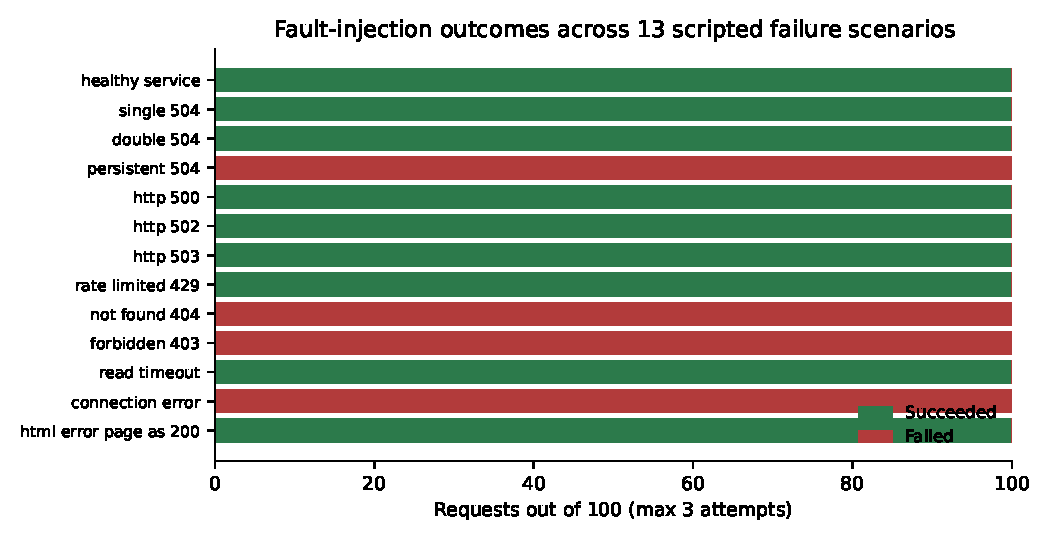
\includegraphics[width=0.92\textwidth]{figures/fault_injection}
\caption{Outcome of 1{,}300 simulated requests across 13 scripted failure
scenarios (100 repeats each). Every scenario behaved exactly as specified:
transient failures (single/double 504, 500/502/503, rate-limited 429, read
timeout, and the HTML-error-page-as-200 case) recovered in 100/100 repeats;
persistent 504 and connection-error scenarios were correctly unrecoverable
at the configured retry budget in 100/100 repeats; permanent errors (404,
403) were correctly not retried, requiring exactly one attempt in 100/100
repeats. Aggregated over the ten scenarios involving a transient or
permanent fault, 1{,}000 of 1{,}300 requests began with a failure, of which
800 (80.0\%) ultimately recovered -- the remaining 200 being the scenarios
designed to be unrecoverable.}
\label{fig:fault-injection}
\end{figure}

\subsection{Performance benchmarking}
\label{sec:performance}

Local (network-independent) computational performance was measured on the
reference machine described in Table~\ref{tab:environment}, from a fixed
random seed, and is reported separately from any measurement involving an
external service: remote response time is a property of the queried
resource, varies with time of day and geography, and is reported instead,
on its own terms, in Section~\ref{sec:live-benchmark}.

\begin{table}[htbp]
\centering
\small
\caption{Reference measurement environment for the performance figures in
this section (Section~\ref{sec:performance}); recorded automatically by the
benchmark script and included here for reproducibility.}
\label{tab:environment}
\begin{tabular}{@{}ll@{}}
\toprule
Python & CPython 3.12.3 \\
Platform & Linux x86-64 \\
Alignment cap & $4\times10^{6}$ dynamic-programming cells \\
\bottomrule
\end{tabular}
\end{table}

Single-sequence analysis completes in 0.47\,ms for a 300\,nt nucleotide
sequence, 4.1\,ms for 3{,}000\,nt, and 45.0\,ms for 30{,}000\,nt; protein
analysis completes in 0.45\,ms, 1.3\,ms, and 4.0\,ms for 100, 300, and
1{,}000 residues respectively. Batch throughput and its scaling with batch
size are shown in Figure~\ref{fig:performance}: per-sequence cost varies by
a factor of 1.16 from a batch of 10 to a batch of 1{,}000 sequences (1.10\,ms
to 1.27\,ms), indicating that throughput (786--912 sequences per second
across this range) is effectively linear in batch size over three orders of
magnitude, rather than degrading with larger batches. Semi-global alignment
cost (Section~\ref{sec:validation}), shown in Figure~\ref{fig:alignment},
scales with the dynamic-programming cell count as expected of the
underlying $O(mn)$ algorithm, from 0.59\,ms for a 76-residue query (the
length of ubiquitin) to 54.1\,ms for a 600-residue query. A cache read
(Section~\ref{sec:caching}) of a representative 200\,kB coordinate payload
completes in 0.21\,ms, roughly four orders of magnitude faster than a
typical remote structure-retrieval request (Section~\ref{sec:live-benchmark}).
Process start-up, from interpreter launch through import and a first
completed sequence analysis, takes 25.5\,ms.

\begin{figure}[htbp]
\centering
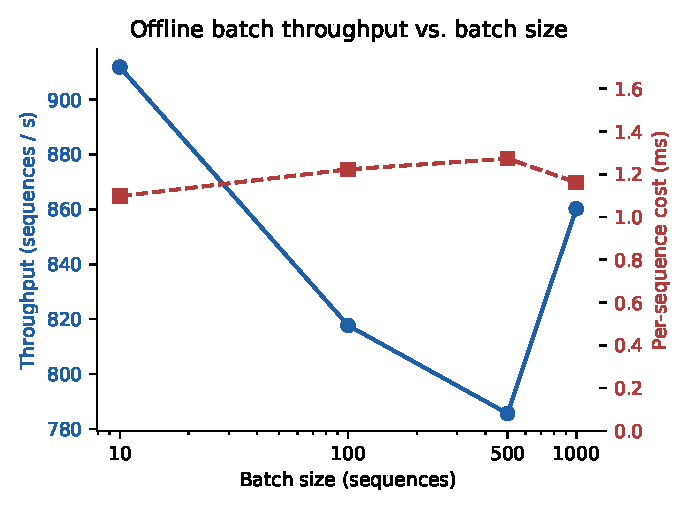
\includegraphics[width=0.62\textwidth]{figures/performance}
\caption{Offline batch-processing throughput (left axis, solid) and
per-sequence cost (right axis, dashed) as a function of batch size, on a
logarithmic horizontal axis. Per-sequence cost is stable across three orders
of magnitude in batch size.}
\label{fig:performance}
\end{figure}

\begin{figure}[htbp]
\centering
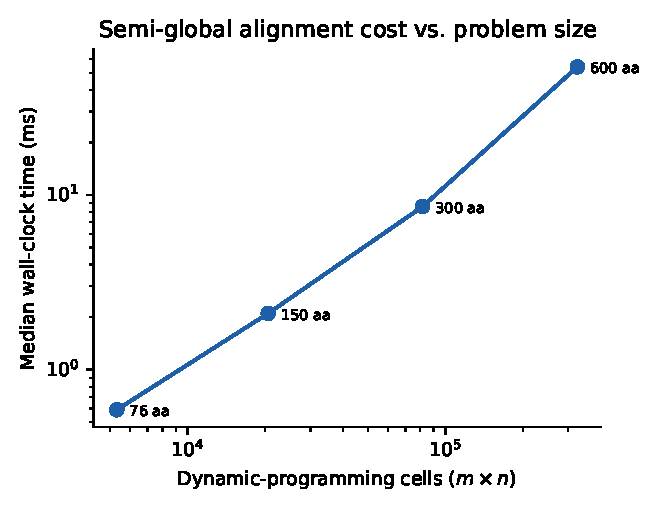
\includegraphics[width=0.55\textwidth]{figures/alignment_scaling}
\caption{Semi-global pairwise alignment (Section~\ref{sec:validation}) cost
as a function of the dynamic-programming problem size, log--log axes,
labelled by query length. Points fall close to a line of slope 1 on
log--log axes, consistent with the expected $O(mn)$ scaling.}
\label{fig:alignment}
\end{figure}

\subsection{Workflow integration}
\label{sec:workflow-comparison}

The claim that an integrated tool reduces effort relative to a manual,
multi-tool workflow is evaluated objectively rather than asserted: for five
representative tasks, a manual workflow using named, freely available web
tools is documented as an explicit, numbered list of steps (available in
full in the software repository, Section~\ref{sec:availability}), and the
number of interaction steps, distinct applications used, and manual
copy-paste data transfers between tools is counted directly from that
documented protocol -- a count that does not depend on the authors' own
software and can be independently checked or disputed against the published
step list. \bsi's equivalent step count is measured the same way against
the actual interface. This method deliberately measures interaction cost,
not human completion time or error rate, for which see the discussion of
usability evidence in Section~\ref{sec:discussion}.

\begin{table}[htbp]
\centering
\small
\caption{Interaction-cost comparison, manual multi-tool workflow versus
\bsi, across five representative tasks. T3's manual step count is the
per-sequence manual protocol (T1, 16 steps) applied across 50 sequences plus
4 batch-level steps ($50 \times 16 + 4 = 804$); \bsi's step count for T3 is
independent of the number of sequences.}
\label{tab:workflow}
\begin{tabular}{@{}p{5.4cm}rrr@{}}
\toprule
\textbf{Task} & \textbf{Manual} & \textbf{\bsi} & \textbf{Reduction} \\
\midrule
T1: single-sequence characterisation & 16 & 3 & 81.2\% \\
T2: structure retrieval with identity check & 17 & 3 & 82.4\% \\
T3: batch of 50 sequences & 804 & 3 & 99.6\% \\
T4: reproduce an earlier analysis & 6 & 3 & 50.0\% \\
T5: hand off to a collaborator & 6 & 2 & 66.7\% \\
\midrule
\textbf{Total} & \textbf{849} & \textbf{14} & \textbf{98.4\%} \\
\bottomrule
\end{tabular}
\end{table}

Table~\ref{tab:workflow} and Figure~\ref{fig:workflow} summarise the
result: across the five tasks, the documented manual workflow requires 849
steps in total against 14 for \bsi\ (98.4\% reduction), spans 16 distinct
applications against 2, and involves 17 manual copy-paste data transfers
between tools against 2. Task T2 is the task most directly relevant to this
paper's central claim: the manual protocol's steps 8--13 (extracting a
retrieved structure's chain sequence and explicitly aligning it against the
query before accepting the result) are the steps a manual workflow most
readily skips under time pressure, and skipping them is mechanistically
the failure mode measured in Section~\ref{sec:validation-study}. In
\bsi, this comparison is not an optional step a user might omit: it is
performed automatically and its result (Table~\ref{tab:m0m4}) is always
shown.

\begin{figure}[htbp]
\centering
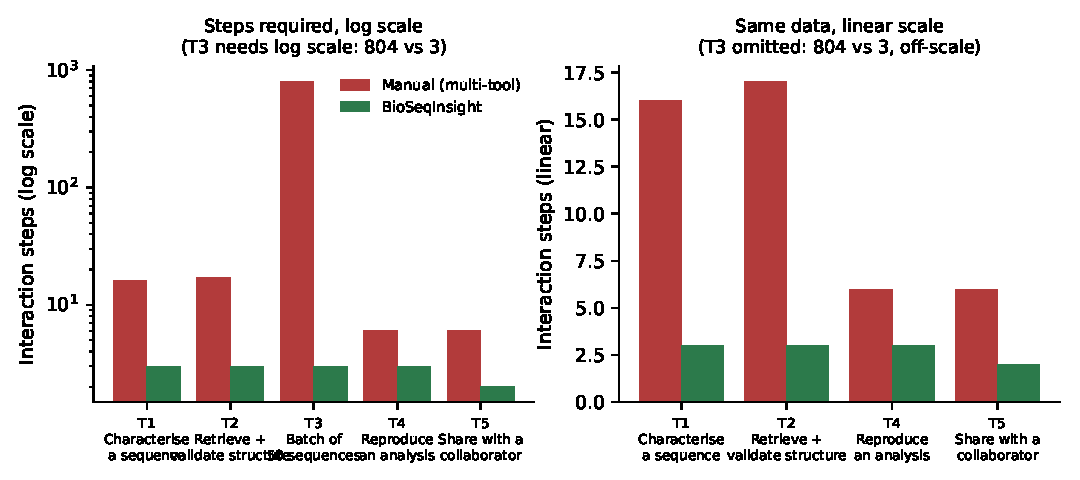
\includegraphics[width=0.92\textwidth]{figures/workflow_comparison}
\caption{Interaction steps required per task, manual multi-tool workflow
versus \bsi. Left: all five tasks, logarithmic axis (required because T3's
manual step count, 804, is two orders of magnitude larger than the
remaining tasks). Right: the same data for the four tasks whose manual step
counts do not require log scaling, linear axis.}
\label{fig:workflow}
\end{figure}

\subsection{Live service benchmark on a curated set}
\label{sec:live-benchmark}

This earlier benchmark exercises the three live services end to end (availability, latency, retrieval success) over a
curated set of 69 proteins (\texttt{benchmarks/data/benchmark\_candidates.csv}
in the software repository) selected specifically to include cases under
which naive, unvalidated structure retrieval is most likely to mislead:
near-identical paralogues (e.g.\ haemoglobin $\alpha$/$\beta$, HRas/KRas),
cross-species orthologues, a bacterial chaperonin/co-chaperonin pair
deposited together, proteins with intrinsically disordered regions,
membrane receptors deposited only as isolated domains, tandem-repeat and
precursor proteins whose deposited structures cover only a fragment of the
full-length sequence, and the human preproinsulin query that the prototype
flagged (Section~\ref{sec:case-study}). The candidate list records accession,
protein name, organism, and functional class, but deliberately \emph{not} a
pre-recorded sequence length: length, and the short/medium/long stratum
derived from it, are fetched from UniProt at benchmark run time rather than
typed in by a curator, so that a reported stratum can never silently
disagree with the sequence actually analysed.

Of the 69 candidates, 69 resolved successfully against UniProt (0
unresolved). Table~\ref{tab:livebench} and Figures~\ref{fig:livebench}--
\ref{fig:mapping} report the outcome of querying all three resources for
every resolved candidate (i.e.\ without early termination at the first
exact match, so that every resource's independent performance is visible).

\begin{table}[htbp]
\centering
\small
\caption{Live structure-resource benchmark, 69 resolved candidate proteins,
all three resources queried for every candidate. \emph{Attempted success
rate} restricts the denominator to requests actually sent (excluding
sequences ESM Atlas refuses before any request for exceeding its configured
length limit), separating genuine service unreliability from candidates a
resource cannot be asked about at all. Run captured
\texttt{2026-09-23}; software version 2.0.2; full per-protein results and
the run's internal consistency checks are included in the software
repository (Section~\ref{sec:availability}).}
\label{tab:livebench}
\begin{tabular}{@{}lrrrrr@{}}
\toprule
\textbf{Resource} & \textbf{Retrieved} & \textbf{Success} & \textbf{Attempted} & \textbf{M4 exact} & \textbf{Median} \\
 & \textbf{/ 69} & \textbf{rate} & \textbf{success rate} & \textbf{matches} & \textbf{response} \\
\midrule
RCSB PDB           & 59 & 85.5\% & 85.5\%  & 39 & 4.98\,s \\
AlphaFold DB       & 68 & 98.6\% & 98.6\%  & 68 & 0.31\,s \\
ESM Atlas          & 46 & 66.7\% & 100.0\% & 0 (predicted) & 2.04\,s \\
\bottomrule
\end{tabular}
\end{table}

\begin{figure}[htbp]
\centering
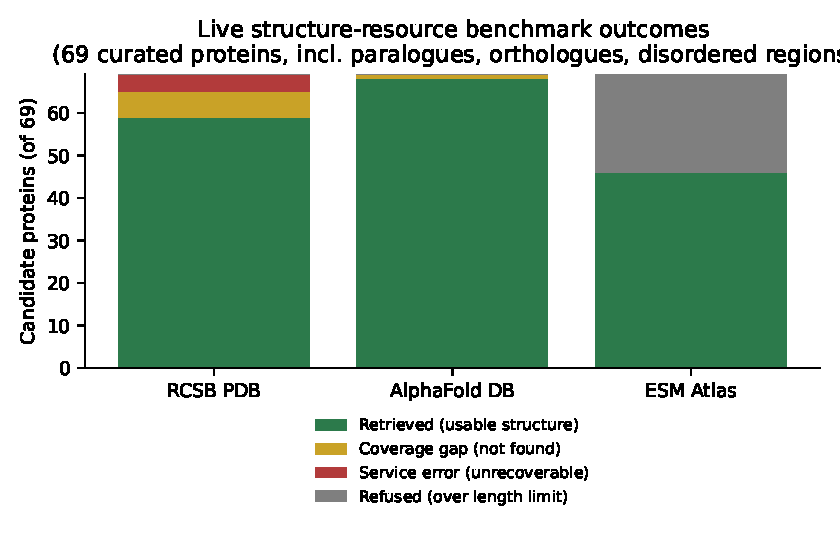
\includegraphics[width=0.72\textwidth]{figures/live_benchmark}
\caption{Outcome category per resource, live benchmark over 69 curated
proteins. ESM Atlas's 23 ``refused'' candidates are sequences exceeding its
configured length limit (400 residues), rejected before any network
request is made and reported as their own category rather than merged into
either successful retrieval or service failure.}
\label{fig:livebench}
\end{figure}

\begin{figure}[htbp]
\centering
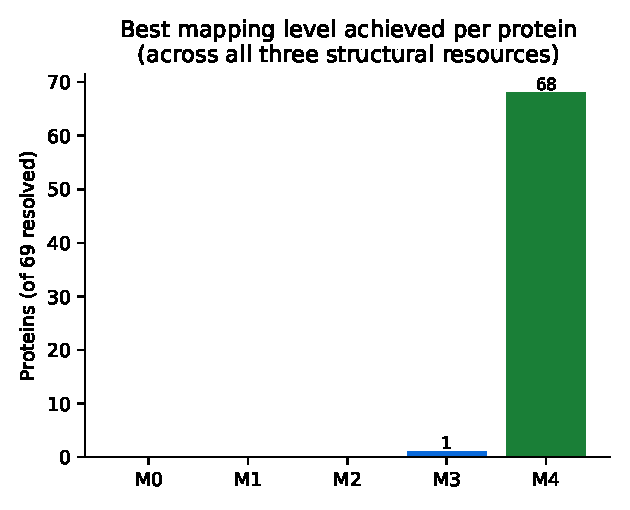
\includegraphics[width=0.5\textwidth]{figures/mapping_distribution}
\caption{Best sequence-to-structure correspondence level achieved per
protein, across all three resources (Table~\ref{tab:m0m4}). Every one of
the 69 candidates achieved at least an M3 classification; 68 (98.6\%)
achieved M4, the level supporting an unqualified statement that the
retrieved structure is the queried protein.}
\label{fig:mapping}
\end{figure}

Combining across resources, 68 of 69 candidates achieved M4 and the
remaining one M3. This figure must be read for what it is: AlphaFold DB is keyed
by UniProt accession, so its model is the queried entry by construction and
reaches M4 almost automatically; the figure is a measure of \emph{service
coverage}, not evidence that validation separates right from wrong structures,
which is the question of Section~\ref{sec:validation-study}. AlphaFold DB's
retrieval rate (98.6\%) reflects the API-discovery design of
Section~\ref{sec:retrieval}: an earlier implementation that constructed the
model file URL from an assumed, fixed model-version number achieved 0\%
retrieval on this identical candidate set once the database had been republished
under a later version -- every request returned HTTP 404, indistinguishable in
isolation from genuine absence of coverage. The comparison illustrates that a
structure-retrieval client's reliability depends on verifying assumptions against
the resource's authoritative interface, not only on the plausibility of its
request construction.


\subsection{Validation study: how often does naive retrieval return the wrong structure?}
\label{sec:validation-study}

\paragraph{Design.}
\emph{Dataset.} We sampled \N{ds-n} reviewed (Swiss-Prot) UniProt entries from
release \N{ds-release}, stratified into four equal length classes (50--150,
150--300, 300--600 and $>$600 residues) with a fixed random seed, by drawing at
random from the complete list of accessions in each class (an earlier version of
the sampler took the first results returned by the search and yielded a sample
that was entirely human; it was corrected before any result was collected). The
sample covers \N{ds-orgs} organisms, the most frequent being \emph{Homo sapiens}
at \N{ds-toporg-pct}\%. Of the \N{ds-n} proteins, \N{ds-has} have at least one PDB
entry cross-referenced in UniProt and \N{ds-no} have none; the sample is
stratified by length and category and is therefore not a representative sample of
the proteome, so rates are comparisons between policies on this set, not
estimates of prevalence.

\emph{Ground truth.} A retrieved PDB entry is judged correct for a query if the
curated databases say it contains a chain mapped to the queried accession. We
require two sources to agree: the PDBe SIFTS UniProt mapping of the entry
\citep{dana2019sifts}, and the reference-sequence identifiers RCSB
attaches to any polymer entity of the entry. Agreement gives a positive label,
joint disagreement a negative one, and a conflict is excluded as ambiguous.
Neither source is \bsi's alignment, so a correct label is not merely the
classifier restating its own output. The label is an \emph{accession-level}
claim: an identical sequence filed under a different accession is negative, and
the two sources are not independent of the cross-references the accession check
reads (Section~\ref{sec:m0m4}).

\emph{Policies.} For each query we took (i) the top RCSB sequence-search hit
with no identity filter, accepted unconditionally; (ii) the top hit of a search
carrying RCSB's own 0.9 identity cutoff, accepted unconditionally; (iii) the
\emph{same} hit as (i) accepted only if \bsi\ classifies it M4 (strict) or M3 or
better (permissive); and (iv) \bsi's own end-to-end retrieval, strict or
permissive. Policy (iii) isolates the value of the validation layer by judging
the same candidate with and without it. AlphaFold DB is accession-keyed and ESM
Atlas predicts from sequence, so neither can return a wrong accession and the
comparison is made on RCSB. The unit of analysis is the query protein. Because
\N{ds-no} proteins have no deposited structure, accepting \emph{any} structure for
them is a false association by definition; the two strata are therefore
reported separately and never blended into one headline.

\paragraph{Results.}
Table~\ref{tab:naive} and Figure~\ref{fig:outcomes} give the outcome of each
policy. Accepting the top sequence-search hit returned a structure not
catalogued under the queried accession for \N{n1-all-false} of \N{n1-all-q}
queries (\N{n1-all-far}\% of the \N{n1-all-acc} accepted hits; 95\% CI
\N{n1-all-far-lo}--\N{n1-all-far-hi}\%). For the \N{ds-has} proteins that have a
deposited structure the figure was \N{n1-has-false} of \N{n1-has-acc} returned
hits (\N{n1-has-far}\%, 95\% CI \N{n1-has-far-lo}--\N{n1-has-far-hi}\%); for the
\N{ds-no} proteins that have none, \N{n1-no-false} of \N{n1-no-acc} returned hits
(\N{n1-no-far}\%), as expected. RCSB's own identity cutoff narrows the problem
but does not remove it: \N{n2-all-false} false associations remain, \N{n2-has-false}
of \N{n2-has-acc} hits (\N{n2-has-far}\%) among proteins that have a structure.

\begin{table}[htbp]
\centering
\footnotesize\setlength{\tabcolsep}{3pt}
\caption{Outcome of five acceptance policies on \N{ds-n} proteins, judged against
curated cross-references. \emph{False} is an accession-level false association.
Sensitivity is the fraction of the \N{ds-has} proteins with a deposited structure
for which a correct structure was returned.}
\label{tab:naive}
\begin{tabular}{@{}lrrrrrrr@{}}
\toprule
 & \multicolumn{3}{c}{All \N{ds-n} queries} & \multicolumn{2}{c}{Structure exists} & \multicolumn{1}{c}{None exists} & \\
\cmidrule(lr){2-4}\cmidrule(lr){5-6}\cmidrule(lr){7-7}
\textbf{Policy} & \textbf{Accepted} & \textbf{False} & \textbf{Rate (95\% CI)} & \textbf{False/acc.} & \textbf{Sens.} & \textbf{False/acc.} & \textbf{FP/1000} \\
\midrule
Naive, top hit & \N{n1-all-acc} & \N{n1-all-false} & \N{n1-all-far}\% (\N{n1-all-far-lo}--\N{n1-all-far-hi}) & \N{n1-has-false}/\N{n1-has-acc} & \N{n1-has-sens}\% & \N{n1-no-false}/\N{n1-no-acc} & \N{n1-all-per1000} \\
Naive, RCSB 0.9 cutoff & \N{n2-all-acc} & \N{n2-all-false} & \N{n2-all-far}\% (\N{n2-all-far-lo}--\N{n2-all-far-hi}) & \N{n2-has-false}/\N{n2-has-acc} & \N{n2-has-sens}\% & \N{n2-no-false}/\N{n2-no-acc} & \N{n2-all-per1000} \\
Validated, permissive (M3+) & \N{p1-all-acc} & \N{p1-all-false} & \N{p1-all-far}\% (\N{p1-all-far-lo}--\N{p1-all-far-hi}) & \N{p1-has-false}/\N{p1-has-acc} & \N{p1-has-sens}\% & \N{p1-no-false}/\N{p1-no-acc} & \N{p1-all-per1000} \\
Validated, strict (M4) & \N{s1-all-acc} & \N{s1-all-false} & \N{s1-all-far}\% (\N{s1-all-far-lo}--\N{s1-all-far-hi}) & \N{s1-has-false}/\N{s1-has-acc} & \N{s1-has-sens}\% & \N{s1-no-false}/\N{s1-no-acc} & \N{s1-all-per1000} \\
End-to-end, strict (M4) & \N{s3-all-acc} & \N{s3-all-false} & \N{s3-all-far}\% (\N{s3-all-far-lo}--\N{s3-all-far-hi}) & \N{s3-has-false}/\N{s3-has-acc} & \N{s3-has-sens}\% & \N{s3-no-false}/\N{s3-no-acc} & \N{s3-all-per1000} \\
\bottomrule
\end{tabular}
\end{table}

\begin{figure}[htbp]
\centering
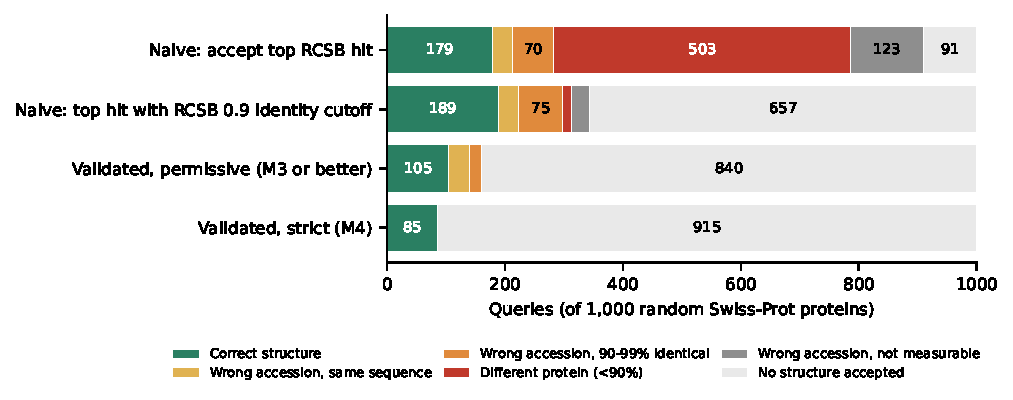
\includegraphics[width=0.95\textwidth]{figures/val_outcomes}
\caption{Outcome of four acceptance policies over all \N{ds-n} queries. False
associations are split by the measured identity of the returned hit to the query:
the same sequence under another accession, 90--99\% identical, a different
protein ($<$90\%), or not measurable (no PDB-format coordinate file exists).}
\label{fig:outcomes}
\end{figure}

\paragraph{What the false associations are.} ``False'' here means not catalogued
under the queried accession, which includes a sequence that is identical but
filed under another accession. We therefore classify each false association by
the hit's own measured identity and coverage. Of the \N{n1-all-false} naive false
associations, \N{n1-all-tier-same} are the same sequence under another accession (for
example identical histone sequences deposited under different accessions),
\N{n1-all-tier-near} are 90--99\% identical, \N{n1-all-tier-diff} are a clearly different
protein ($<$90\% identity), and \N{n1-all-tier-unm} could not be measured because the
entry has no PDB-format file. The permissive policy leaves \N{p1-all-false} false
associations, of which \N{p1-all-tier-same} are the same sequence and
\N{p1-all-tier-near} near-identical, and \emph{none} is a different protein
(\N{p1-all-tier-diff}). Among proteins that have a structure, the naive policy's
\N{n1-has-false} false associations comprise \N{n1-has-tier-same} same-sequence,
\N{n1-has-tier-near} near-identical, \N{n1-has-tier-diff} different-protein and
\N{n1-has-tier-unm} unmeasurable hits. The substantive failure of naive retrieval
is therefore real but smaller than the headline: most false associations are
proteins without any structure, for which a homologue is returned, and a minority
of those for proteins with a structure are clearly the wrong molecule.

\paragraph{The validation layer.} Accepting only M4 produced \N{s1-all-false}
false associations among \N{s1-all-acc} accepted structures (95\% CI
\N{s1-all-far-lo}--\N{s1-all-far-hi}\%), and \bsi's end-to-end strict policy
accepted \N{s3-all-acc} with \N{s3-all-false}. An exact McNemar test on the
per-query false-association outcome, naive versus strict on the same hit, has
\N{disc-n1-s1} discordant queries in one direction and none in the other
($p = \N{p-n1-s1}$), and the comparison against RCSB's cutoff policy is
\N{disc-n2-s2} versus 0 ($p = \N{p-n2-s2}$); because every discordance goes one way
these tests add little beyond the counts. Two cautions apply. The accession
component of the check and the ground truth both read curated cross-references,
so a zero here shows consistency between two views of related curated data, not
an independent audit. And unmeasurable hits cannot be accepted, so part of the
reduction is the refusal to accept what could not be checked.

\paragraph{The cost.} The strict policy returned a correct structure for
\N{s1-has-sens}\% of the proteins that have one, against \N{n1-has-sens}\% for the
naive policy (Table~\ref{tab:naive}). Figure~\ref{fig:gatecost} accounts for the
correct naive hits it did not accept: of \N{gate-total} correct hits, \N{gate-accepted}
were accepted and \N{gate-rejected} rejected, of which \N{gate-partial} were partial
structures of the right protein (accession confirmed, identity $\geq$95\%,
coverage $<$80\%), \N{gate-unmeasured} could not be validated because RCSB serves
no PDB-format file for the entry (large and recent assemblies; every case was an
HTTP 404), \N{gate-m3} were M3 (accession not confirmed) and \N{gate-other}
fell in M1 or M2. The permissive policy recovers part of this at the price of
\N{p1-all-false} false associations (none a different protein), reaching
\N{p1-has-sens}\% sensitivity. The choice between operating points is therefore a
trade-off the user can make knowingly: strict M4 for a claim that the structure
\emph{is} this protein; permissive M3+ when the same or a near-identical sequence
is acceptable.

\begin{figure}[htbp]
\centering
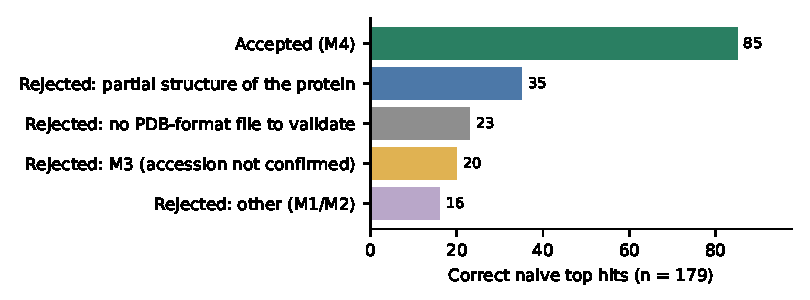
\includegraphics[width=0.78\textwidth]{figures/val_gate_cost}
\caption{What the strict (M4) policy did with the correct top hits returned by
naive retrieval. Partial structures are real structures of the queried protein
that are not full length; the partial-structure qualifier now labels them.}
\label{fig:gatecost}
\end{figure}

\subsection{Adversarial benchmark}
\label{sec:adversarial}

To test the validator on cases built to fool it, we constructed negatives from
the dataset and passed each (query, forced structure) pair directly through the
validation function, independently of any search. Table~\ref{tab:adversarial} and
Figure~\ref{fig:adversarial} report the outcome. In total \N{adv-total} cases were
built and \N{adv-scored} could be resolved and scored; the rest (\N{adv-unresolved})
had no retrievable forced structure and are excluded, which means the scored cases
are not a random subset of those built.

\begin{table}[htbp]
\centering
\small
\caption{Adversarial benchmark. Each case is a query with a forced structure
that is wrong in a specified way. Levels are the validator's output; \emph{partial}
counts results flagged as partial structures.}
\label{tab:adversarial}
\begin{tabular}{@{}p{4.4cm}rrrrrrr@{}}
\toprule
\textbf{Class (construction)} & \textbf{Scored} & \textbf{M1} & \textbf{M2} & \textbf{M3} & \textbf{M4} & \textbf{Partial} \\
\midrule
B1 wrong paralogue (same Pfam family, est.\ 40--95\% identity) & \N{adv-B1-n} & \N{adv-B1-M1} & \N{adv-B1-M2} & \N{adv-B1-M3} & \N{adv-B1-M4} & \N{adv-B1-partial} \\
B2 fragment of the right protein (SIFTS coverage $<$70\%) & \N{adv-B2-n} & \N{adv-B2-M1} & \N{adv-B2-M2} & \N{adv-B2-M3} & \N{adv-B2-M4} & \N{adv-B2-partial} \\
B4 unrelated protein (random pairing) & \N{adv-B4-n} & \N{adv-B4-M1} & \N{adv-B4-M2} & \N{adv-B4-M3} & \N{adv-B4-M4} & \N{adv-B4-partial} \\
B5 near-identical, different entry & \N{adv-B5-n} & \N{adv-B5-M1} & \N{adv-B5-M2} & \N{adv-B5-M3} & \N{adv-B5-M4} & \N{adv-B5-partial} \\
B3 other isoform (labels unverified) & \N{adv-B3-n} & \N{adv-B3-M1} & \N{adv-B3-M2} & \N{adv-B3-M3} & \N{adv-B3-M4} & \N{adv-B3-partial} \\
\bottomrule
\end{tabular}
\end{table}

\begin{figure}[htbp]
\centering
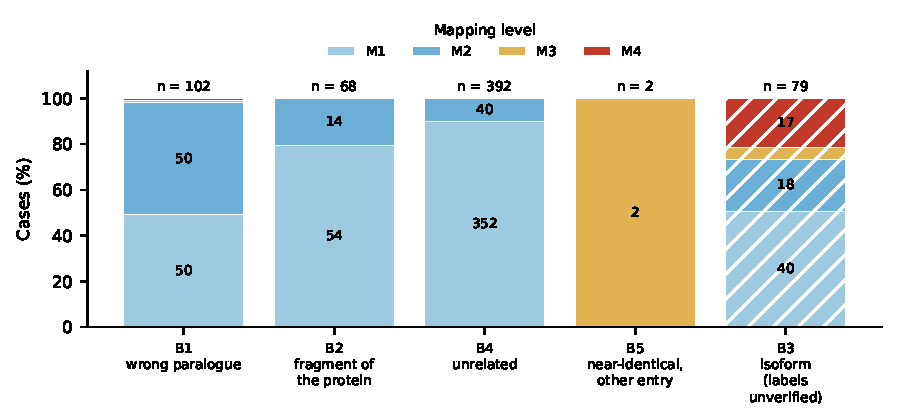
\includegraphics[width=0.78\textwidth]{figures/val_adversarial}
\caption{Mapping level reached by each adversarial class (counts shown in the
bars). Hatched: B3, whose ``wrong isoform'' label is a construction assumption
rather than ground truth.}
\label{fig:adversarial}
\end{figure}

None of the \N{adv-B4-n} unrelated pairs and none of the \N{adv-B2-n} fragments
reached M4 (or M3). Of the \N{adv-B1-n} paralogue pairs, \N{adv-B1-M1} fell to M1, \N{adv-B1-M2} to M2,
\N{adv-B1-M3} to M3 and \N{adv-B1-M4} reached M4; B5 has only \N{adv-B5-n} scored
cases and supports no conclusion. Across B1, B2, B4 and B5,
\N{adv-nonB3-M4} of \N{adv-nonB3-n} cases reached M4. A case that does reach M4
necessarily has a confirmed accession, identity $\geq$99\% and coverage $\geq$95\%,
so the forced ``paralogue'' structure in fact contains the queried protein; we
treat such a pair as a construction error (a Pfam-paired entry that is the same
protein) rather than a validator failure, but this benchmark cannot distinguish
that from an error in the cross-reference, and the case is reported, not excluded.

Two results are informative beyond the counts. First, the unrelated pairs are not
all at M1: \N{adv-B4-M2} of \N{adv-B4-n} (\N{adv-B4-M2-pct}\%) reached M2, which
Section~\ref{sec:threshold} shows is the noise floor of the alignment, not a
detection of homology. Second, B2 exposed the message defect of
Table~\ref{tab:defects}: the \N{adv-B2-accconf} fragments whose accession is
confirmed are real structures of the queried protein, yet fell to M1 or M2 with a
warning that they do not correspond to it; \N{adv-B2-partial} are now flagged as
partial structures; the others do not meet the qualifier's bounds (identity
$\geq$95\%, coverage $<$80\%), and we have not examined them individually. B3 is not interpreted as a failure rate: an isoform that
differs from the canonical sequence by a small region yields a structure that
legitimately matches the canonical query, so its ``wrong isoform'' label is not
ground truth. Restricting to the \N{adv-B3-valid-n} cases whose isoform is more than
5\% shorter than the canonical sequence (a rule fixed before the outcomes were
inspected), \N{adv-B3-valid-M4} reached M4. The adversarial set was built by a
script whose pair ordering depended on string-hash order; the file used here is
frozen and its checksum recorded, but regenerating it gives a different sample.

\subsection{Identity, coverage and accession: where the thresholds are meaningful}
\label{sec:threshold}

We used the same hits to ask which of the three measurements carries the
discrimination. Positives are the naive hits that ground truth labels correct
(\N{auc-n-npos}); negatives are the naive hits it labels wrong
(\N{auc-n-nneg}) or, separately, constructed unrelated, paralogue and
near-identical negatives (\N{auc-a-nneg}). Table~\ref{tab:auc} gives the area under
the ROC curve for identity, coverage and their product.

\begin{table}[htbp]
\centering
\small
\caption{Area under the ROC curve for separating correct hits from wrong ones.}
\label{tab:auc}
\begin{tabular}{@{}lrrrr@{}}
\toprule
\textbf{Negatives} & \textbf{n (pos/neg)} & \textbf{Identity} & \textbf{Coverage} & \textbf{Identity $\times$ coverage} \\
\midrule
Wrong naive hits & \N{auc-n-npos}/\N{auc-n-nneg} & \N{auc-n-id} & \N{auc-n-cov} & \N{auc-n-ic} \\
Constructed negatives & \N{auc-a-npos}/\N{auc-a-nneg} & \N{auc-a-id} & \N{auc-a-cov} & \N{auc-a-ic} \\
\bottomrule
\end{tabular}
\end{table}

Coverage does not add discrimination; the product scores \emph{worse} than
identity alone. The reason is that correct hits include many fragments, which
have low coverage and are the right protein: coverage measures completeness, not
whether the molecule is right. What removes the high-identity wrong hits is the
accession check. At the M4 identity and coverage thresholds (identity
$\geq$\N{th-exact-identity}\%, coverage $\geq$\N{th-exact-coverage}\%),
\N{abl-neg-ic} of \N{abl-neg} negatives would be accepted on identity and coverage
alone, and \N{abl-neg-ica} survive the accession check; of \N{abl-pos} correct
hits, \N{abl-pos-ic} pass identity and coverage and \N{abl-pos-all} pass all three.

\paragraph{The M2 threshold sits at the noise floor.} Because identity is
measured over the aligned region only, unrelated pairs can look similar by
chance. Over the \N{nf-n} unrelated pairs the median identity is \N{nf-p50-all}\%
and the 90th percentile \N{nf-p90-all}\%, but \N{nf-hilow} of these pairs reach
$\geq$50\% identity at coverage below the related threshold, a short-subject
artefact. Conditioning on coverage $\geq$\N{th-related-coverage}\%
(n = \N{nf-n-cov}) the 99th percentile identity is \N{nf-p99-cov}\%.
\N{nf-m2} of \N{nf-n} unrelated pairs (\N{nf-m2-pct}\%) satisfy the M2 criteria
(identity $\geq$\N{th-related-identity}\%, coverage $\geq$\N{th-related-coverage}\%),
\N{nf-id50} reach 50\% identity at that coverage, and \N{nf-high} reach the M3
criteria and \N{nf-exact} the M4 criteria. M2 therefore must not be read as evidence of
homology; M3 and M4 lie well above the floor. We did not retune the M2 threshold
on these data, because doing so on the evaluation set would overfit; a held-out
calibration is future work. Figure~\ref{fig:grid} shows the two joint
distributions.

\begin{figure}[htbp]
\centering
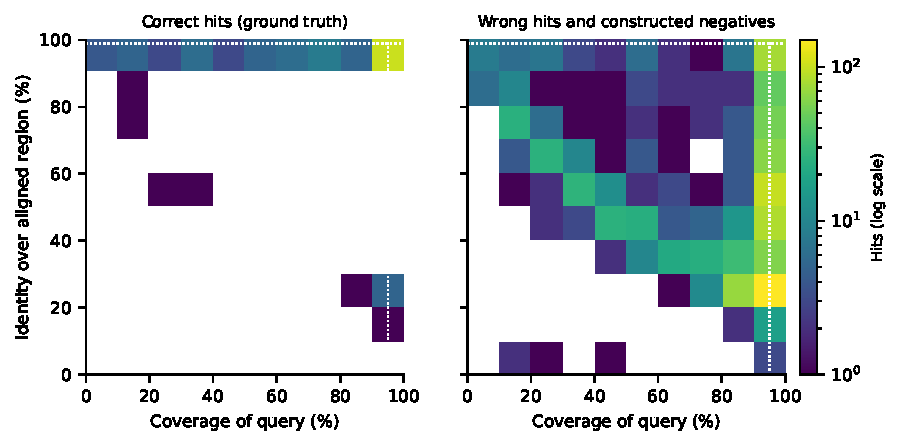
\includegraphics[width=0.9\textwidth]{figures/val_grid}
\caption{Hits by identity and coverage (10-point bins, log colour scale): correct
hits (left) concentrate at high identity and coverage, with a tail of partial
structures at high identity and low coverage; wrong hits and constructed
negatives (right) follow a diagonal in which identity rises as coverage falls.
Dotted lines mark the M4 thresholds.}
\label{fig:grid}
\end{figure}

\subsection{Re-adjudicating the 25-protein prototype benchmark}
\label{sec:case-study}

The 25 queries of the v1.0 prototype benchmark, quoted from its Table~3, were
re-run against current data (\texttt{validation/scripts/06\_case\_studies.py}). For
each, we took the top RCSB sequence-search hit, judged whether its entry
contains the queried accession (the 76-residue ubiquitin sequence, encoded
identically by four genes, counts any of them), and validated it. This reproduces
what a sequence-based retrieval returns \emph{today}; it cannot recover what v1.0
retrieved in August 2026, as the archive has changed since. Table~\ref{tab:discordance}
gives the outcome.

\begin{table}[htbp]
\centering
\small
\caption{Top RCSB sequence-search hit for the 25 prototype queries, by whether the
prototype's own report flagged an accession discordance.}
\label{tab:discordance}
\begin{tabular}{@{}lrrrrrr@{}}
\toprule
\textbf{Prototype flag} & \textbf{n} & \textbf{Entry contains accession} & \textbf{Ambiguous} & \textbf{M4} & \textbf{M3} & \textbf{$<$M3} \\
\midrule
Discordant (``mapped $\ldots$'') & \N{cs-disc-n} & \N{cs-disc-contains} & \N{cs-disc-amb} & \N{cs-disc-M4} & \N{cs-disc-M3} & \N{cs-disc-low} \\
Not flagged & \N{cs-oth-n} & \N{cs-oth-contains} & \N{cs-oth-amb} & \N{cs-oth-M4} & \N{cs-oth-M3} & \N{cs-oth-low} \\
\bottomrule
\end{tabular}
\end{table}

For \N{cs-disc-contains} of the \N{cs-disc-n} flagged queries the top hit is an
entry that contains the queried accession, and \N{cs-disc-M4} validate as M4.
The prototype's discordances therefore do not show that it retrieved wrong
structures; they show an attribution problem (the accession reported for a hit was
not always the accession of the queried chain, for example in multi-chain
complexes). Among the \N{cs-oth-n} unflagged queries, \N{cs-oth-contains} top hits
contain the accession, \N{cs-oth-amb} is ambiguous (the two curated sources
disagree), and \N{cs-oth-low} validate below M3, which shows that a hit can contain
the right accession and still be a poor structural match to the full sequence.
\textbf{This study does not support the claim that the prototype returned wrong
structures}; it motivates the larger measurement of
Section~\ref{sec:validation-study}.


\section{Discussion}
\label{sec:discussion}

\subsection{What this evidence supports}

The evaluation in Section~\ref{sec:evaluation} addresses three separable claims,
and it is worth stating precisely what supports each. \emph{Maturity} is
supported by the test suite, the continuous-integration matrix and the packaging
evidence of Sections~\ref{sec:testing} and~\ref{sec:package-architecture}; the six
defects in Table~\ref{tab:defects} are offered as evidence that testing was
substantive, not that the software is defect-free, which no finite suite can
establish. \emph{Reliability} is supported at two levels that should not be
conflated: behaviour under network failure (Section~\ref{sec:fault-injection}, a
controlled deterministic experiment) and the correctness of the \emph{output},
where the central evidence is the validation study of
Section~\ref{sec:validation-study}. \emph{Value over an unintegrated manual
workflow} is supported by an objective interaction-cost comparison
(Section~\ref{sec:workflow-comparison}), which is a proxy for effort, not a
measurement of human task time or error rate.

\subsection{What validation buys, and what it costs}

The validation study separates two things that a single ``success'' flag
conflates. Accepting the top sequence-search hit returns a structure not
catalogued under the queried accession for most queries in a random sample, but
most of those are proteins that have no deposited structure at all, for which a
homologue comes back; for proteins that do have a structure the naive policy was
wrong for a minority of queries, and a smaller part of those were clearly a
different protein. Validation converts these into explicit levels. The strict
policy accepted no wrong structure, and the permissive policy's false
associations were all the same or a near-identical sequence. The price is
sensitivity: \N{s1-has-sens}\% of proteins with a structure received an M4 against
\N{n1-has-sens}\% for the naive policy, because many correct structures are partial,
cannot be validated, or lack a confirmed accession.

We therefore present the two operating points as a choice, not a verdict. A user
who needs to assert that a structure \emph{is} the queried protein should take M4
and accept that it will often return nothing; a user who can use the same or a
near-identical sequence should take M3 or better; a user who simply wants a
related fold can take any level but should read the level. Partial structures,
now flagged, are real structures of the protein and are often what a
structural biologist wants; the flag lets them be found without weakening M4.

\subsection{The AlphaFold defect as a general lesson}

The AlphaFold DB retrieval defect (Table~\ref{tab:defects};
Section~\ref{sec:live-benchmark}) is discussed not because it was unusually severe
but because of how it presented: a client that built the model URL from an assumed
version number returned HTTP 404 for every request once the database was
republished, which is indistinguishable in isolation from the absence of a model.
The general lesson is that a retrieval client's assumptions about a remote
resource should be verified against its authoritative interface, and that a
failure rate near 100\% on a resource that should have high coverage is itself
a signal. The same applies to this study's own tooling, as the next subsection
records.

\subsection{Verifying the verifier}

The validation study itself went wrong in ways that are instructive, and we
report them because the same errors are easy to make in any benchmark of a
validation layer. Our first analysis scored the naive baselines as accepted
exactly when their hit was correct and then evaluated them against that same
label, which made them perfect by construction. Our first threshold analysis
defined its ``true positives'' as the classifier's own M4 output, which made the
separation circular. An early sampler took the first results returned by a search
and produced an all-human sample. The adversarial set was built with an ordering
that depended on string hashing, so a ``seeded'' draw differed between runs. A
documentation table stated thresholds that did not match the shipped defaults.
Each was found by inspecting the output against what it should have been, was
corrected before the numbers reported here were produced, and is logged as a
protocol amendment in the repository. The practical conclusion is that a
benchmark of a verification step needs the same adversarial scrutiny as the step.

\subsection{Why the classification generalises, and where it does not}

The M0--M4 design is deliberately resource-agnostic: it depends only on a query
sequence, a returned chain, and optionally a set of cross-references, so it applies
unchanged to experimental structures, accession-keyed predictions and
sequence-only predictions. Its strongest levels depend on cross-references that
only some resources provide, which is why ESM Atlas predictions cannot reach M4 by
design. Its weakest level, M2, depends on an identity measure that is not
discriminating at the threshold we ship (Section~\ref{sec:threshold}); a user
should treat M2 as a prompt to look, not as a finding.

\section{Limitations}
\label{sec:limitations}

\paragraph{Ground truth is accession-level and not fully independent.} Correctness
is judged against PDBe SIFTS and RCSB entity references. These are curated
independently of the software's alignment, but they are not independent of the
cross-references the accession check reads, so a result of zero false associations
at M4 shows consistency between two views of related curated data, not an
independent audit. A structure that is the right protein but catalogued under a
different accession is counted as a false association; the tiering of
Section~\ref{sec:validation-study} shows how much of the total this is, but the
headline rates should be read as accession-level.

\paragraph{The sample is not representative.} The \N{ds-n} proteins are a random
draw from reviewed UniProt entries, stratified by length and category, taken at one
time from one release. About \N{ds-no} of \N{ds-n} have no deposited structure,
which is typical of Swiss-Prot, and the rates are comparisons between policies on
this set, not estimates of prevalence in any user's workload.

\paragraph{Entries without a PDB-format file cannot be validated.} The RCSB
provider downloads PDB-format files, which do not exist for large or recent
entries. \N{gate-unmeasured} of the \N{gate-total} correct naive hits and
\N{n1-all-tier-unm} of the \N{n1-all-false} naive false associations could not be
validated for this reason (every case an HTTP 404). They cannot be accepted, which
costs sensitivity. Validating from the polymer-entity sequence when no PDB file
exists is a bounded fix we have not made.

\paragraph{M2 is not evidence of homology.} The related-record thresholds sit at the
alignment's noise floor: \N{nf-m2-pct}\% of unrelated pairs satisfy them
(Section~\ref{sec:threshold}). We did not retune them on the evaluation data.
Identity is computed over the aligned region only and is inflated for short
subject chains.

\paragraph{The strict policy has low sensitivity.} A correct structure was
returned for \N{s1-has-sens}\% of proteins that have one. Most of the loss is
legitimate (partial structures, no file to validate), but a user who needs
coverage must use the permissive operating point and accept its same-sequence and
near-identical false associations.

\paragraph{The adversarial benchmark is limited and partly unverified.} B5 has only
\N{adv-B5-n} scored cases. B1 depends on a Pfam grouping and a crude sequence-similarity
estimate used only for construction, and a pair that reaches M4 is most likely a
construction error that this benchmark cannot distinguish from a cross-reference
error. B3's label is an assumption, not ground truth, and is not reported as a
failure rate. \N{adv-unresolved} of \N{adv-total} built cases could not be scored,
so the scored cases are not a random subset. The frozen set was produced by a
script whose pair ordering was not reproducible, so regenerating it gives a different sample.

\paragraph{The 25-protein re-adjudication reproduces today's archive, not the
prototype's.} It cannot show what v1.0 retrieved in August 2026, only what a
sequence search returns now. It shows the prototype's discordance flags do not
demonstrate wrong structures; it does not show what the prototype did.

\paragraph{The live service benchmark is small and its M4 rate is a coverage figure.}
The 69-protein set was curated to include difficult cases and AlphaFold DB is
accession-keyed, so its M4 rate says nothing about validation. Service behaviour
varies with time; the dated runs retained in the repository document that variation.

\paragraph{Fault injection and usability.} The 80\% recovery figure is a property
of the injected scenarios, not an expected service-level rate. Interaction-step
counts are a proxy for effort; no human-subject usability study has been run, and
the protocol for one is included in the repository. The statement-coverage figure,
the standalone installer and the archival DOI are pending
(\todoinline{insert \texttt{pytest --cov} output, installer status and Zenodo DOI}).

\paragraph{Scope.} Structure retrieval covers a single query chain; multi-chain
assemblies are validated by their best-matching chain, and complexes in which the
queried protein is one of many chains are classified on that chain only.

\section{Conclusions}
\label{sec:conclusions}

We presented \bsi\ 2.0, an integrated platform for sequence analysis and protein
structure retrieval whose distinguishing feature is that every retrieved structure
is checked against the query and reported on an explicit five-level scale, with a
qualifier for confirmed but partial structures. On \N{ds-n} randomly sampled
proteins, judged against independently curated cross-references, accepting the top
sequence-search hit returned a structure not catalogued under the queried accession
for \N{n1-all-false} queries, including \N{n1-has-false} of \N{n1-has-acc} hits for
proteins that have a structure; accepting only M4 accepted \N{s1-all-false} wrong
structures, at the cost of returning a correct structure for \N{s1-has-sens}\% of
proteins that have one rather than \N{n1-has-sens}\%. The main reasons for that cost
are partial structures and entries that cannot be validated from a PDB-format file,
both addressable.

The same study qualifies the claim. Zero false associations at M4 is consistency
between two views of related curated data; the false associations that remain
at the permissive level are the same or a near-identical sequence; M2 is not
evidence of homology; and the prototype's accession discordances do not
demonstrate wrong structures. The software and the measurement are released
together, with the protocol amendments that record how the measurement was
corrected, so that the validation layer and the benchmark that tests it can both
be scrutinised.

\section{Software and data availability}
\label{sec:availability}

\bsi\ is released under the MIT licence. Source code, the complete test
suite, all benchmark scripts and their outputs (including every dated live
benchmark run referenced in Section~\ref{sec:live-benchmark}, retained as an
audit trail, and the validation package that produces Sections~\ref{sec:validation-study}--\ref{sec:case-study}), the documented manual-workflow protocol
(Section~\ref{sec:workflow-comparison}), the usability-study protocol
referenced in Section~\ref{sec:limitations}, and full documentation are
available at:

\begin{center}
\url{https://github.com/niloy-999/BioSeqInsight}
\end{center}

\noindent The version described in this manuscript is tagged
\texttt{v2.0.2} and archived with a permanent identifier at
\todoinline{Zenodo DOI: 10.5281/zenodo.XXXXXXX -- mint on first GitHub
Release from the v2.0.2 tag, after connecting the repository to Zenodo, and
insert the resulting DOI here before submission.} An earlier prototype
(v1.0.0), discussed for context in Sections~\ref{sec:introduction} and
\ref{sec:case-study}, is preserved unmodified at the repository tag
\texttt{v1.0-archive}.

\paragraph{Installation.}
\begin{lstlisting}
pip install bioseqinsight
\end{lstlisting}
requires Python 3.10 or later and no compiled dependencies
(Section~\ref{sec:package-architecture}). \todoinline{If a standalone
installer (Section~\ref{sec:limitations}) is available at submission time,
add its location here.}

\paragraph{Reproducing the results in this paper.}
Every quantitative result in Section~\ref{sec:evaluation} is produced by a
script included in the repository under \texttt{benchmarks/scripts/}, runnable
independently of this manuscript:

\begin{lstlisting}
git clone https://github.com/niloy-999/BioSeqInsight.git
cd BioSeqInsight && pip install -e ".[validation]"

python -m pytest --cov=bioseqinsight            # Section 5.1-5.2
python benchmarks/scripts/run_fault_injection.py         # Section 5.3
python benchmarks/scripts/run_performance_benchmark.py   # Section 5.4
python benchmarks/scripts/run_workflow_comparison.py     # Section 5.5
python benchmarks/scripts/run_structure_benchmark.py \
    --out benchmarks/results/structure_benchmark_$(date +%F)  # live service benchmark, network

# validation study (network; about a day): see validation/README.md
bash validation/run_all.sh baselines
bash validation/run_all.sh threshold
bash validation/run_all.sh casestudies
bash validation/run_all.sh report
python validation/scripts/07_manuscript_numbers.py   # every number in Sections 5.6-5.9
\end{lstlisting}

The validation study depends on the state of UniProt, RCSB and PDBe at run time
and on a frozen adversarial case file whose SHA-256 is recorded beside it; the
protocol, its amendments and the corrected analyses are in
\texttt{validation/PROTOCOL.md}. The three benchmarks not requiring network access
(Sections~\ref{sec:fault-injection}--\ref{sec:workflow-comparison}) are
deterministic and reproduce the reported figures exactly on any machine; the
live structure-resource benchmark (Section~\ref{sec:live-benchmark}) depends
on the queried resources' state at run time and is expected to vary modestly
between runs, as documented by the multiple dated runs retained in the
repository during this software's development.

\paragraph{Data availability.} No new biological data were generated. The
live benchmark candidate list
(\texttt{benchmarks/data/benchmark\_candidates.csv}) references public
UniProt accessions only; all retrieved structures originate from the public
resources cited in Section~\ref{sec:retrieval} and are subject to those
resources' own terms of use.


\section*{Acknowledgments}
\todoinline{Add any acknowledgments (colleagues who piloted the software,
institutional computing resources, etc.), or delete this section if none.}

\section*{Funding}
\todoinline{State funding sources, or explicitly ``This work received no
specific funding.''}

\section*{Author contributions}
\todoinline{CRediT taxonomy statement, e.g. Conceptualization, Software,
Validation, Writing -- original draft, Writing -- review \& editing, etc.,
attributed to each author.}

\section*{Conflict of interest}
The authors declare no competing interests.

\bibliography{references}

\end{document}
